\documentclass[dm,ppgcomp]{texfurg}
\usepackage[utf8x]{inputenc}
\usepackage[T1]{fontenc}
\usepackage{graphicx}
\usepackage{algorithmic}
\usepackage{algorithm}
\usepackage{placeins}
\usepackage{natbib}

\setlength{\emergencystretch}{18pt}

\title{Uma proposta de algoritmo para o Modelo AB de dobramento de proteínas}

\advisor[Prof.]{Machado}{Karina dos Santos}
\coadvisor[Prof.]{Emmendorfer}{Leonardo}
\author{Couto}{Rafael Castro do}

\keyword{Javascript}
\keyword{Dobramento de proteí­na}
\keyword{Bioinformática}
\keyword{Modelo AB}

\renewcommand{\date}{\today}

\begin{document}

\maketitle

\begin{abstract}

O problema de dobramento de proteínas continua presente como um desafio na área de Bioinformática. Com o objetivo de entender alguns aspectos desse problema, a comunidade científica tem proposto uma série de modelos altamente simplificados, porém não triviais. 
Este trabalho utiliza um modelo de polímero contínuo simplificado que incorpora características estruturais essenciais e considera as interações entre os aminoácidos chamado Modelo AB. Este modelo foi desenvolvido para explorar a adaptação de redes neurais na predição de padrões de dobramento de proteínas na forma de estrutura primária (sequência de aminoácidos). Atualmente existem diferentes implementações para a solução do dobramento de proteínas com o uso do Modelo AB que despendem um longo tempo de execução em máquinas de alta performance. 
O algoritmo desenvolvido incorpora soluções inspiradas nos algoritmos de estimação de distribuição e em estratégias de aprendizagem de máquina para a busca da solução ótima. Essa solução utiliza dois conceitos principais: Rigidez e Eficiência para gerar novas dobras e utiliza ainda conceitos das meta-heurísticas de {\it Simulated Annealing} para executar o refinamento dos dobramentos obtidos.
Sendo assim, o presente trabalho trabalho propõe uma nova abordagem para a solução do problema de dobramento de proteínas utilizando o Modelo AB. Para a validação do algoritmo proposto, os resultados obtidos são comparados com trabalhos relacionados. Para a execução dessas comparações, foi desenvolvida uma aplicação em $JavaScript$. A partir dos resultados obtidos, espera-se que a abordagem apresentada neste trabalho possa ser aplicada no desenvolvimento de novos algoritmos para dobramento de proteínas reais ou para a solução de outros problemas relacionados. 

\end{abstract}

\begin{englishabstract}
{An implementation of the AB model in a web application}
{Javascript, Protein Folding, Bioinformatic, AB Model}

The protein folding problem continues to present scientific challenges in the area of Bioinformatic. In an effort to understand a few aspects of protein folding, the scientific community has proposed several highly simplified, but still non trivial models. 
The present paper concerns a model of continuum polymer models that incorporate simplified backbone potentials and inter amino acids interactions called AB Model. It was developed to explore the adaptation of neural networks to prediction of folding patterns of proteins from their primary structure (amino acid sequence along the backbone). Several modern implementations that aim to solve the protein folding problem through the AB Model take a long execution time even on high performance machines.  
The developed algorithm incorporates solutions inspired by distribution estimation algorithms and machine learning strategies for searching the optimal solution. This solution uses two main concepts: Rigidity and Efficiency to generate new folds and also uses concepts of Simulated Annealing meta-heuristics to perform folds refinement.
Thus, the present work proposes a new approach to solving the problem of protein folding through the AB Model. In order to validate the proposed algorithm, the results achieved are compared with related works. To perform this comparisons, an application was developed in $JavaScript$. It is expected that the content can help on the development of new tools to deal with the protein folding problem and other related problems.

\end{englishabstract}

%Lista de Figuras
\listoffigures

%Lista de Tabelas
\listoftables

%lista de abreviaturas e siglas
\begin{listofabbrv}{SPMD}

\item[ACMC] Annealing Contour Monte Carlo
\item[ANN] Algoritmo Proposto inspirado no Simulated Annealing 
\item[API] Application Programming Interface
\item[BOA] Bayesian Optimization Algorithm
\item[BMDA] Bivariate Marginal Distribution Algorithm
\item[CASP] Critical Assesment od Structural Prediction
\item[cGA] Compact Genetic Algorithm
\item[CSA] Conformational Space Annealing
\item[FDA] Factorized Distribution Algorithm
\item[EcGA] Extended compact Genetic Algorithm
\item[EDA] Estimation of Distribution Algorithm
\item[ELA] Estimation Learning Algorithm (Algoritmo Proposto)
\item[HTS] Heuristic-based Tabu Search
\item[JS] JavaScript
\item[MIMIC] Mutual Information Maximization for Input Clustering
\item[PBIL] Population-Based Incremental Learning
\item[RAM] Random Access Memory
\item[SA] Simulated Annealing
\item[STMD] Statistical Temperature Molecular Dynamics
\item[UMDA] Univariate Marginal Distribution Algorithm

\end{listofabbrv}

%Sumario
\tableofcontents

\chapter{Introdução}

Entre as diversas áreas da Biologia, uma das que mais se beneficia das ferramentas computacionais e da Bioinformática é a Biologia Molecular. O estudo dos seres vivos em uma escala molecular está em evidência devido aos avanços científicos nos últimos anos, principalmente na área da Genética \cite{mount2004sequence}.

A Genética é o estudo da hereditariedade e mostra a importância de conhecer ao nível molecular os genes. É através dos processos de transcrição e tradução dos genes que as células produzem cadeias polipeptídicas, também denominadas proteínas. As proteínas são muito importantes e participam na maior parte dos processos celulares \cite{hunter1993molecular}.

A estrutura primária de uma proteína é a sua sequência de aminoácidos e de acordo com Anfinsen \cite{anfinsen1973principles}, essa estrutura pode determinar a conformação final da proteína. A partir desta sequência, a proteína se dobra e toma sua forma final denominada conformação nativa. Apesar das proteínas não serem moléculas totalmente rígidas, a função que elas vão exercer no sistema biológico é determinada pela sua forma. 

Apesar de existirem muitas pesquisas com o objetivo de prever o dobramento de proteínas, ainda não existe um método computacional que encontre a conformação nativa para qualquer proteína-alvo rapidamente. Isso se deve ao fato dessa previsão, frequentemente denominada problema de dobramento de proteínas, ser consideravelmente complexa \cite{fraenkel1993complexity}.

Com o objetivo de facilitar o a busca por novas soluções para este complexo problema de dobramento de proteínas foram desenvolvidos modelos simplificados \cite{stillinger1993toy}. Esses modelos mantém as características relevantes das proteínas e reduzem a demanda computacional para a busca da solução, além de agilizar a implementação de novas soluções. Este trabalho utiliza um destes modelos simplificados denominado Modelo AB. Nesse modelo, os aminoácidos são simplicados sendo resumidos a somente dois tipos: $A$ hidrofóbicos e $B$ hidrófilos.

Diversos algoritmos foram implementados com o objetivo de prever a conformação de menor energia de uma proteína-alvo no Modelo AB. Dentre eles destacam-se os Algoritmos Genéticos, Redes Neurais \cite{stillinger1995collective}, {\it Simmulated Annealing} (SA) e os Algoritmos de Distribuição Estimada (EDA). 

O objetivo deste trabalho é propor um novo algoritmo para o dobramento de proteínas utilizando o Modelo AB. O algoritmo proposto neste trabalho se inspira nos algoritmos SA, EDAs e em técnicas de Aprendizagem de Máquina. Para coordenar a execução das novas soluções, de forma que elas trabalhem em conjunto formando uma heurística que explora de forma inteligente o espaço de busca, foi implementada uma aplicação {\it web}.

Tanto as heurísticas e técnicas de aprendizagem de máquina quanto os algoritmos de otimização podem ser implementados através de diferentes tecnologias. Uma  possibilidade interessante do ponto de vista do desenvolvimento consiste na implementação utilizando tecnologias da {\it internet}. Nessa tecnologias, o código em $JavaScript$ (JS) é interpretado, o que simplifica o desenvolvimento.

Os algoritmos foram implementados utilizando a linguagem de programação JS, incluindo as estruturas virtuais das proteínas simplificadas, os cálculos da energia e a aplicação para testes. Através dessa aplicação, que faz a interface com o usuário, foram gerados gráficos do espaço de soluções para tetrâmeros, simulações das estruturas, os gráficos do comportamento da energia ao longo da busca e os gráficos finais.

No Capítulo 2, são apresentados resumidamente os conceitos relevantes ao problema, dentre eles podemos citar os diferentes níveis estruturais das proteínas, a abrangente área de estudos da Bioinformática, a classe de complexidade do problema e o modelo adotado neste trabalho. 

Os trabalhos que serviram de base para o desenvolvimento do algoritmo são relacionados no Capítulo 3, com o objetivo de detalhar a evolução do problema e de seus modelos. Nesse capítulo é analisada a busca da comunidade científica pela solução do problema, os modelos simplificados mais conhecidos e os algoritmos relevantes já desenvolvidos para o dobramento de proteínas no Modelo AB utilizados na comparação com os resultados do algoritmo proposto.

Em seguida, encontram-se os dois algoritmos propostos (ANN e ELA) e sua análise, desde os conceitos que serviram de inspiração para cada um, como foram desenvolvidos até a sua implementação. Os conceitos de Eficiência e Rigidez aplicados no algoritmo ELA são analisados detalhadamente em gráficos nessa seção.

A seção 4.3 descreve como foi implementada a aplicação que gerencia os testes e apresenta os resultados. Finalmente apresentamos as análises dos resultados obtidos e dos parâmetros utilizados para chegar a esses resultados. Apesar desta proposta ser recente seus resultados são animadores.

\chapter{Referencial Teórico}

\section{Bioinformática}

Bioinformática pode ser considerada uma área de conhecimento multidisciplinar que envolve uso intensivo de ferramentas computacionais. Nessa área, os computadores são usados para resolver problemas na área de ciências biológicas, envolvendo principalmente a manipulação de grandes bancos de dados, como sequências de nucleotídeos, sequências de proteínas, estruturas de proteínas, entre outros \cite{mount2004sequence}. De forma complementar, também envolve técnicas como modelagem tridimensional de proteínas e de outros sistemas biológicos, estudos de filogenia, desenho racional de fármacos, etc. De forma resumida, a Bioinformática tem como objetivos principais a coleta, organização, armazenamento, recuperação e análise de dados biológicos, propiciando a inferência ou descoberta de informações sobre a biologia e/ou evolução dos organismos \cite{luscombe2001bioinformatics}.

Inúmeros projetos transnacionais de grande importância, por exemplo, o Projeto Genoma Humano, se destacam no campo da Bioinformática. No Brasil, existem também  inúmeros projetos que envolvem tanto o sequenciamento, quanto análises genômicas e/ou proteômicas de organismos que provocam patogenias. Como por exemplo o sequenciamento genético da bactéria {\it Xylella fastidiosa} \cite{simpson2000genome}.

Um dos problemas mais importantes dentro da área de Bioinformática e Biologia computacional que continua em aberto é a predição do dobramento de proteínas. Conferências são realizadas em diversos países para tratar especificamente desse problema e das pesquisas que objetivam sua solução. Um desses eventos é denominado CASP ({\it Critical Assesment od Structural Prediction}) e é realizado a cada dois anos reunindo diversos pesquisadores para uma competição. Nesta competição, os pesquisadores recebem sequências de proteínas que tiveram sua estrutura resolvida em laboratório, porém não foram publicadas. Vence o grupo que conseguir prever {\it ab initio}, com maior precisão, a estrutura do maior número de sequências \cite{prosdocimi2002bioinformatica}.

Para propor novos algoritmos para o dobramento de proteínas é necessário um entendimento aprofundado sobre o problema. Para isso, na próxima seção deste trabalho, é apresentando o conceito de proteínas e suas estruturas. 

\section{Proteínas}

Os papéis que as proteínas desempenham nos sistemas biológicos são muito diversos: catálise de reações, transporte, suporte e movimento, resposta imunitária, entre outros. A proteína representada nas Figuras \ref{seq} e \ref{1ahoimg} é identificada pelo código PTB ID 1AHO \cite{berman2000protein}. A Figura \ref{1ahoimg} mostra essa proteína em sua estrutura terciária, é nesta forma que a proteína exerce sua função. 

\begin{figure}[htbp]
  \centering 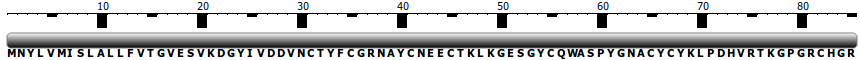
\includegraphics[scale=0.6]{img/seq.png}
\caption{Sequência primária da proteína PTB ID 1AHO.} 
\label{seq}
\end{figure}

Uma proteína pode ser definida como um polímero linear composto por aminoácidos ou como um composto orgânico constituído por um ou mais polipeptídeos. Os aminoácidos são moléculas orgânicas que se unem através de ligações peptídicas, formando os peptídeos e a estrutura primária da proteína. Os aminoácidos são de diversos tipos e sua classificação é extensiva, podendo ser classificados quanto ao radical e quanto às suas propriedades.

Os aminoácidos são moléculas constituídas por um átomo de carbono ($C$) central (designado carbono alfa), um átomo de hidrogénio ($H$), um grupo carboxilo ($COOH$), um grupo amina ($NH2$) e uma cadeia lateral (grupo $R$) conforme a Figura \ref{amino}.

\begin{figure}[htbp]
  \centering 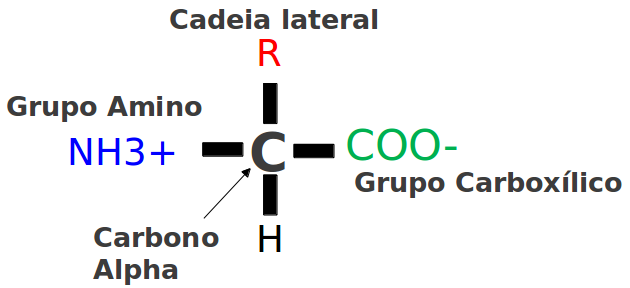
\includegraphics[scale=0.4]{img/amino.png}
\caption{Moléculas que compõem um aminoácido.} 
\label{amino}
\end{figure}

A relação entre os aminoácidos e as moléculas de água ($H2O$) é uma propriedade muito importante para o entendimento deste trabalho. Essa relação pode ser positiva, ou de atração, para os aminoácidos hidrófilos ou pode ser oposta para os hidrofóbicos. Os aminoácidos hidrófilos podem ser divididos em polares com carga positiva, polares com carga negativa e polares com carga neutra, a pH fisiológico ({\it pH 6-7}), enquanto os hidrofóbicos são classificados como apolares.

Sabe-se que uma proteína pode ser formada por milhares de aminoácidos e sua sequência influencia diretamente na conformação final da proteína \cite{anfinsen1973principles} . A sequência de aminoácidos ao longo da cadeia polipeptídica é denominada estrutura primária, ela pode ser simples e pequena como na Figura \ref{seq} ou, na maior parte dos casos, longa e complexa.

O arranjo espacial de aminoácidos próximos entre si na sequência primária da proteína forma a estrutura secundária, que se caracteriza por duas formações principais: as alfa-hélices (Figura \ref{helice}) e as folhas-beta (Figura \ref{folha}), além de estruturas que não são nem hélices nem folhas, chamadas alças. 

\begin{figure}[htbp]
  \centering 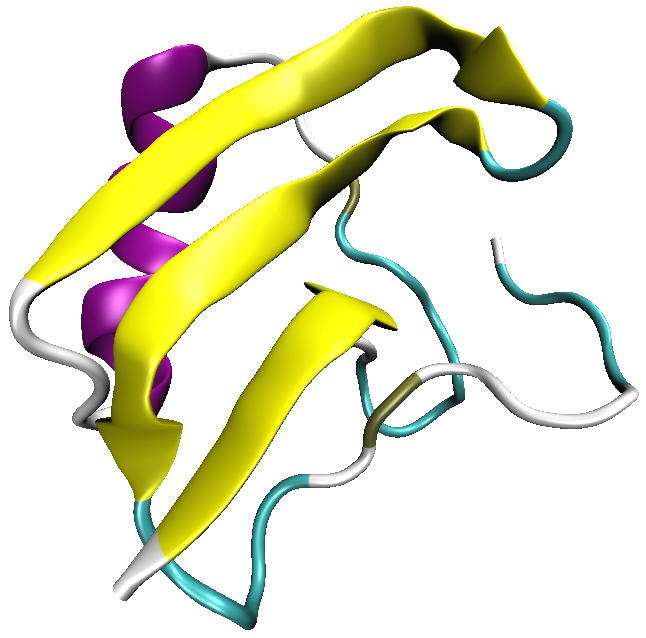
\includegraphics[scale=0.25]{img/1aho.png}
\caption{Estrutura terciária da proteína PDB ID 1AHO.} 
\label{1ahoimg}
\end{figure}

\begin{figure}[htbp]
  \centering 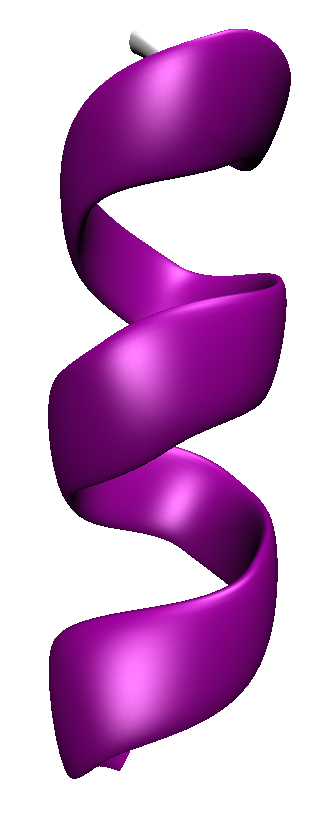
\includegraphics[scale=0.18]{img/helice.png}
\caption{Representação tridimencional de alfa-hélices (estrutura secundária).} 
\label{helice}
\end{figure}

\begin{figure}[htbp]
  \centering 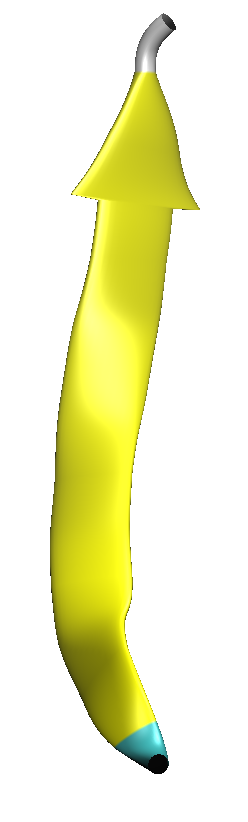
\includegraphics[scale=0.18]{img/folha.png}
\caption{Representação tridimencional de folhas-beta (estrutura secundária).} 
\label{folha}
\end{figure}

Enquanto a estrutura secundária é determinada pelo relacionamento estrutural de curta distância, a terciária (Figura \ref{1ahoimg}) é caracterizada pelas interações de longa distância entre aminoácidos, denominadas interações hidrofóbicas, pelas interações eletrostáticas, pontes de hidrogênio e de sulfeto. Finalmente, algumas proteínas podem ter duas ou mais cadeias polipeptídicas, a conformação dessas cadeias em estruturas tridimensionais é a estrutura quaternária (Figura \ref{1bvrimg}).

Existe a hipótese de que a conformação de uma proteína pode ser determinada a partir da sequência primária, o que permitiria que algoritmos fossem desenvolvidos para predizer estruturas terciárias quando a primária estivesse disponível \cite{anfinsen1973principles}. 

\begin{figure}[htbp]
  \centering 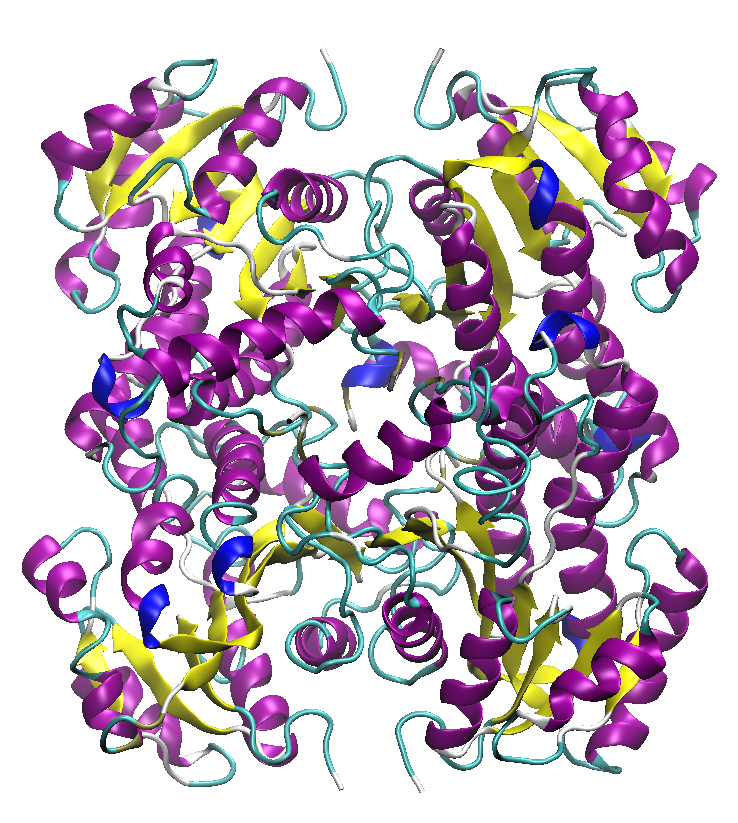
\includegraphics[scale=0.35]{img/1bvr.png}
\caption{Estrutura quaternária da proteína PDB ID 1BRV.} 
\label{1bvrimg}
\end{figure}

A conformação de uma proteína determina sua função, portanto a sequência de aminoácidos pode predizer o comportamento de uma determinada proteína no organismo. Entender como se define a forma de uma proteína (dobramento) é um desafio para a comunidade científica. Porém esta é uma tarefa muito complexa com altas demandas computacionais mesmo para proteínas pequenas. 

Na próxima seção é analisado este complexo processo de dobramento, sua importância e caracterísicas.

\section{Dobramento de Proteínas}

Considerando a importância do processo de dobramento das proteínas para a definição de sua funcionalidade no metabolismo dos organismos, muito esforço tem sido feito na tentativa de compreender seu funcionamento. Apesar de muito conhecimento ter sido gerado, ainda restam muitas perguntas a serem respondidas e esse fato é agravado pelo estudo do genoma humano, que tem aumentado em muito a quantidade de proteínas a serem estudadas \cite{ptitsyn1996determinable} .

A compreensão do processo de dobramento de proteínas é de fundamental importância para a área da saúde, podendo ser utilizado na dedução de relações evolutivas para, por exemplo, a criação de medicamentos inteligentes e para o entendimento de algumas doenças. Dentre essas doenças estão o câncer, fibrose cística, encefalopatia espongiforme bovina (doença da vaca louca), mal de {\it Alzheimer}, mal de {\it Parkinson} e diabetes tipo II, que são causadas por aglomerações de proteínas mal dobradas que não desempenham corretamente sua função e danificam as células saudáveis \cite{dobson1999protein}.

A sequência de aminoácidos específica de uma proteína, também denominada estrutura primária, dobra-se para formar a sua configuração natural. Apesar destas macromoléculas aparentarem estar a dobrar-se a si mesmas, a sua dobra muda de acordo com as características das moléculas que as rodeiam, incluindo enzimas, concentração dos sais, a pressão, a temperatura, enfim de infinitos elementos. O dobramento é um processo espontâneo, natural \cite{anfinsen1973principles}.

A comunidade científica têm estudado muitas proteínas, dobrando-as simultaneamente em larga escala. Percebe-se que na transição para o estado natural, uma dada sequência de aminoácidos percorre, de forma geral, o mesmo caminho, passando pelos mesmos estados intermediários \cite{anfinsen1973principles}.

Pode-se dizer que, o dobramento envolve o estabelecimento de uma estrutura secundária, particularmente hélices-alfa e folhas-beta, e depois uma estrutura terciária. O ponto essencial no dobramento é, no entanto, o fato da sequência de aminoácidos especifica de cada proteína conter a informação que indica a sua conformação final e o caminho para atingir esse estado.

A conformação nativa de uma proteína é frequentemente a configuração termodinamicamente mais estável, ou seja, que possui menor energia livre \cite{anfinsen1973principles}. Assim, podemos descrever o problema de predição de estruturas de proteínas como um problema de otimização, onde a estrutura com menor energia livre deve ser encontrada dentre todas as possíveis estruturas. 

\begin{figure}[htbp]
  \centering 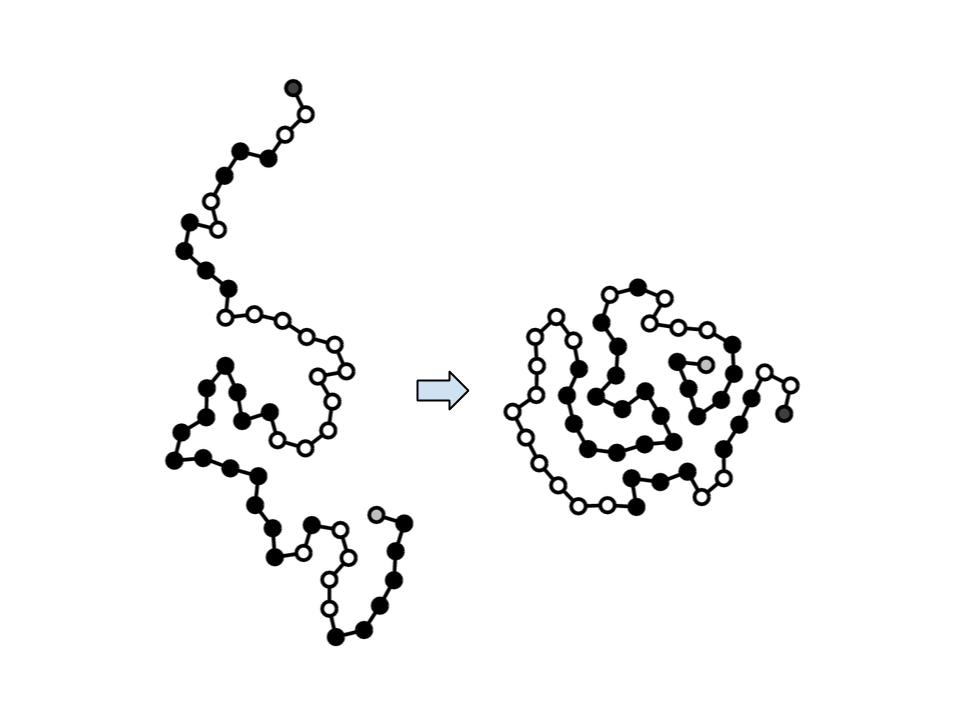
\includegraphics[scale=.35]{img/foldAB.jpg}
\caption{Exemplificação do dobramento no Modelo AB.} 
\label{abfold}
\end{figure}

O problema de dobramento de proteínas pertence a uma classe específica de problemas denominados NP-completos. Esta classe específica de problemas será detalhada na seção 2.6. 

Antes porém, com o objetivo de facilitar o entendimento da complexidade do problema, é analisado o modelo simplificado adotado por este trabalho. Este modelo proposto por Stillinger \cite{stillinger1993toy} em 1993 denominado Modelo AB, torna mais clara a compreenção do problema como um problema de otimização.

\section{Modelo AB}

De forma a desenvolver soluções para o complexo problema do dobramento de proteínas foram desenvolvidos modelos para a descrição de uma proteína de forma simplificada, sendo os mais conhecidos o Modelo HP (Lattice) \cite{stillinger1993toy} e o Modelo AB (Off Lattice) \cite{zhao2008advances}. 

No modelo de dobramento AB, a proteína é descrita como uma sequência de aminoácidos hidrofóbicos ($A$) e hidrófilos ($B$). Apesar de nem todos os aminoácidos serem hidrofóbicos ou hidrófilos, o Modelo AB adota somente estes dois tipos. Muitas propriedades como massa, volume e carga eletromagnética também não são consideradas. 

Esse modelo é uma evolução do Modelo HP, no qual os aminoácidos sofrem as mesmas simplificações. Porém, no Modelo HP, os ângulos são restritos à uma grade ortogonal e nem todas as interações entre aminoácidos contribuem no cálculo da energia \cite{zhao2008advances}.

A Figura \ref{ab} apresenta uma estrutura de proteína simplificada com treze aminoácidos em seu estado mais estável, onde “a” representa o ângulo entre o segundo e o terceiro aminoácidos. No Modelo AB os ângulos são restritos entre ($-\pi, \pi$) radianos, ou seja, entre -180º e + 180º. 

\begin{figure}[htbp]
  \centering 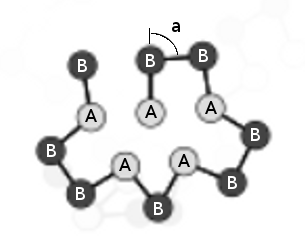
\includegraphics[scale=.55]{img/ab.png}
\caption{Estrutura de proteína bidimensional no Modelo AB.} 
\label{ab}
\end{figure}

Para o cálculo da energia de um modelo de proteína-alvo em uma determinada conformação é utilizada a Equação \ref{energyeq}:

\begin{equation}\label{energyeq}
  E=((1/4)\sum_{i=1}^{(N-2)}(1+cos\theta_{i, i+1}))+4\sum_{i=1}^{(N-2)}\sum_{j=i+2}^{N}(d^{-12}_{i, j}-C (a_{i}, a_{j})d^{-6}_{i, j})$$
Sendo:\\
C (A, A) = 1\\
C (B, B) = 0.5\\
C (A, B) = C (B, A) = -0.5\\
\end{equation}

Onde $E$ representa a energia, $N$ corresponde ao comprimento da sequência de aminoácidos, $a$ é o tipo do aminoácido ($A$ ou $B$), $C$ são as cargas dadas, $\theta$ é o ângulo entre os aminoácidos e $d$ a distância entre os aminoácidos.

O Algoritmo \ref{energyal} demonstra como é calculada a energia de um modelo de proteína AB em uma determinada conformação, dadas as distâncias, as cargas e os ângulos:

\begin{algorithm}
  \caption{Cálculo da energia no Modelo AB}\label{energyal}
  \begin{algorithmic}
  
  \STATE {v1 = 0, v2 = 0}
  \FOR{i = 1; i < (n - 2); i++}
    \STATE {v1 = v1 + (1 + cos(ang[i])) / 4}
  \ENDFOR
  \FOR{i = 0; i < (n - 2); i++}
    \FOR{j = (i + 2); j < n; j++}
      \STATE {v2 = v2 + (4 * (pow(d(i,j), -12) – c(i,j) * pow(d[i][j], -6)))}
    \ENDFOR
  \ENDFOR
  \STATE {energy = v1 + v2}
  \RETURN {energy}
  
  \end{algorithmic}
\end{algorithm}

Existe o Modelo AB tridimensional, que utiliza dois ângulos para definir a posição de cada aminoácido. Esta versão é mais próxima da realidade pois cada resíduo possui as três coordenadas ($x, y$ e $z$), porém o resultado gráfico dos modelos de proteínas obtido é menos legível devido às informações do eixo $z$, conforme a Figura \ref{ab3d}, sendo mais difícil de ser representado e analisado.

\begin{figure}[htbp]
  \centering 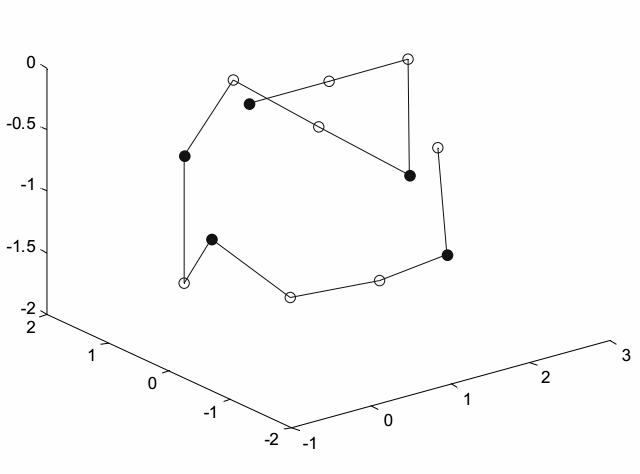
\includegraphics[scale=.45]{img/ab3d.png}
\caption{Estrutura de proteína tridimensional no Modelo AB.} 
\label{ab3d}
\end{figure}

Neste trabalho é utilizado o Modelo AB bidimensional e são utilizadas sequências de aminoácidos adaptadas para este modelo obtidas através da revisão da literatura. Estas sequências são explicadas em detalhes na próxima seção.

\section{Cadeias Primárias no Modelo AB}

As sequências de aminoácidos no Modelo AB, conforme citado anteriormente, são compostas por somente dois tipos de aminoácidos: $A$ e $B$. Inicialmente foram geradas cadeias de acordo com a sequência de Fibonacci \cite{bergum1996applications}, onde o próximo elemento é resultado da concatenação dos últimos dois elementos. O objetivo é evitar padrões repetitivos e simétricos, tornando o modelo mais próximo de uma proteína real. A sequência de Fibonacci segue a forma a seguir:

\begin{equation}\label{fibo}
\[f(0) = 0; f(1) = 1; f(n) = f(n-2) + f(n-1); \]
\[Ex: 0, 1, 1, 2, 3, 5, 8, 13, 21, … \]
\end{equation}

Para adaptar essa sequência ao modelo, a adição é substituida por concatenação. No modelo adotado, conforme mencionado anteriormente, a letra $A$ será utilizada para aminoácidos hidrofóbicos e a letra $B$ para os hidrófilos, portanto as sequências ficam assim:

\begin{equation}\label{fiboab}
\[f(0) = A; f(1) = B; f(n) = f(n-2) + f(n-1); \]
\[Ex: A, B, AB, B AB, AB BAB, BAB ABBAB, … \]
\end{equation}

Nos testes realizados, que são detalhados no Capítulo 5, foram utilizadas quatro sequências de diferentes comprimentos que utilizam a Equação (\ref{fiboab}), estas cadeias estão detalhadas na Tabela \ref{tabelaab}.

\FloatBarrier
\begin{table}
\begin{center}
\caption{Sequências de Fibonacci para o Modelo AB}\label{tabelaab}
\begin{tabular}{l}
\hline
Cadeia - Sequência \\
\hline
FIBO6(13) - ABBABBABABBAB;\\
FIBO7(21) - BABABBABABBABBABABBAB;\\
FIBO8(34) - ABBABBABABBABBABABBABABBABBABABBAB;\\
FIBO9(55) - BABABBABABBABBABABBABABBABBABABBABBABABBABAB\\
\hspace{63 pt}BABBABABBAB;\\
\hline
\end{tabular}
\end{center}
\end{table}

Além dos modelos gerados a partir da série de Fibonacci também são utilizadas duas sequências inspiradas em proteínas existentes, reais. Essas sequências são adaptações de sequências primárias conhecidas e seu objetivo é aproximar ainda mais o modelo de uma situação real, sendo a primeira sequência correspondente à estrutura primária da proteína armazenada no Protein Data Bank (PDB) através da identificação (PDB ID) 1AGT e a segunda identificada como 1AHO \cite{berman2000protein}. 

Para obter as cadeias, os aminoácidos tipo $I, V, L, P, C, M, A$ e $G$ são considerados hidrofóbicos e representados pela letra $A$ e os resíduos $D, E, F, H, K, N, Q, R, S, T, W$ e $Y$ considerados hidrófilos e representados pela letra $B$ \cite{mount2004sequence}. A tabela \ref{tabelareal} mostra a sequência de aminoácidos original de cada estrutura e a sequência correspondente adaptada para o Modelo AB.

\begin{table}
\begin{center}
\caption{Sequências de proteínas reais adaptadas para o Modelo AB}\label{tabelareal}
\begin{tabular}{l}
\hline
Cadeia - Sequência \\
\hline
1AGT(REAL) - GVPINVSCTGSPQCIKPCKDAGMRFGKCMNRKCHCTPK\\
1AGT(AB)\hspace{15 pt} - AAAABABABABABAABAABBAAABBABAABBBABABAB\\
1AHO(REAL) - VKDGYIVDDVNCTYFCGRNAYCNEECTKLKGESGYCQ\\
\hspace{80 pt}WASPYGNACYCYKLPDHVRTKGPGRCH\\
1AHO(AB)\hspace{15 pt} - ABBABAABBABABBBAABBABABBBABBABABBABAB\\
\hspace{80 pt}BABABABAABABBAABBABBBAAABAB\\
\hline
\end{tabular}
\end{center}
\end{table}

Tando as sequências traduzidas para o modelo através de proteínas reais quanto aquelas geradas em função da série de Fibonacci geram modelos que ainda conservam características de proteínas reais, como o surgimento de pequenos padrões de dobra, a formação de núcleos hidrofóbicos compactos e protegidos \cite{fraenkel1993complexity}, entre outros. 

Apesar das simplificações serem consideráveis a solução do problema está longe de ser trivial e apresenta uma alta complexidade. Analisaremos detalhadamente esse grau de complexidade na seção seguinte.

\section{Complexidade do problema no Modelo AB}

O conjunto de problemas que podem ser resolvidos em tempo polinomial por uma máquina de Turing determinística é denominado P, qualquer problema neste conjunto pode ser resolvido por um algoritmo com tempo de execução $O (n^k)$, com $k$ constante \cite{anderson1986machine}.

O conjunto de problemas que são decidíveis em tempo polinomial por uma máquina de Turing não-determinística é denominado NP. Um subconjunto de NP denominado NP-completo é um conjunto cujos problemas precisam satisfazer a seguinte condição: todo problema em NP é redutível para este problema em tempo polinomial. Portanto, se tivéssemos um algoritmo de tempo polinomial para resolver um problema NP-completo, poderíamos resolver todos os problemas NP em tempo polinomial \cite{fraenkel1993complexity}.

Para discutir a complexidade do problema de dobramento de proteínas, foi desenvolvida uma aplicação para mapear o espaço de busca, ou seja, calcular a energia em todas as conformações possíveis de uma proteína simplificada de acordo com o Modelo AB. 

Com o objetivo de gerar gráficos bidimensionais, foram utilizados tetrâmeros, ou seja, cadeias com quatro aminoácidos. O primeiro e o último ângulo não mudam a conformação do modelo de proteína, pois sua alteração não gera uma dobra. Mudar os ângulos das extremidades significa girar toda a proteína. Portanto, o conjunto de todas as possíveis soluções para os tetrâmeros pode ser repesentado como um vetor bidimensional. 

O primeiro ângulo é descrito no eixo vertical ($y$) e o segundo no eixo horizontal ($x$). Os ângulos variam entre $-\pi, \pi$ radianos, de forma que no centro de cada eixo estão os ângulos de valor 0. Portanto o valor do centro de cada gráfico da Figura \ref{space} representa os modelos de proteína em sua conformação linear. 

O valor da energia de cada conformação está apresentado em cores com valores mínimos indicado em cada gráfico através de pontos. Os valores de energia maiores que um (energia > 1) estão em vermelho enquanto os valores menores que um (energia < 1) são graduados linearmente de acordo com a barra de cores;

\begin{figure}[htbp]
  \centering 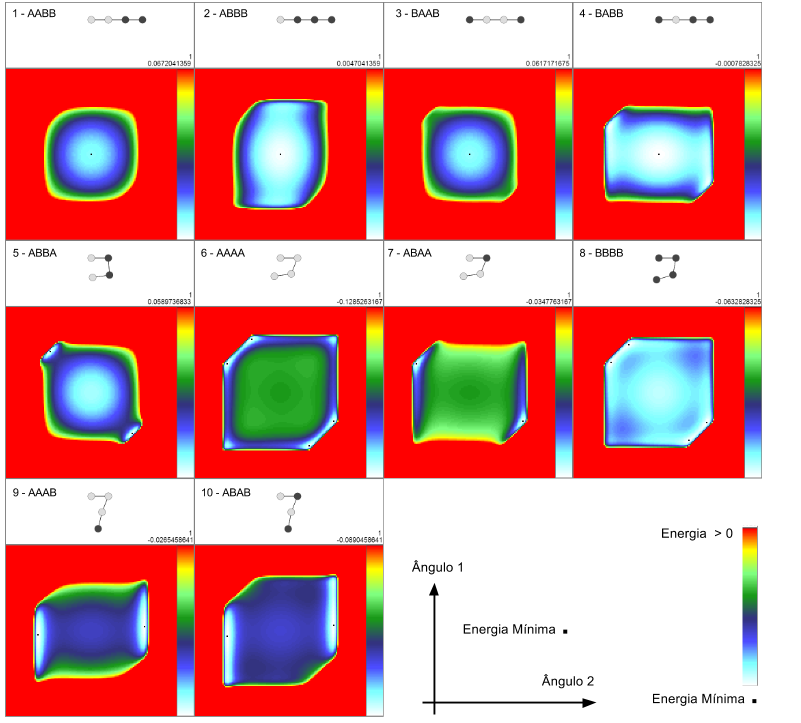
\includegraphics[scale=.55]{img/space.png}
\caption{Espaço de soluções bidimensional para tetrâmeros.} 
\label{space}
\end{figure}

Nos gráficos, mesmo nos modelos cuja solução é linear, a distribuição dos valores de energia é única para cada sequência. Ou seja, apesar de apresentarem a mesma solução ótima, o espaço de soluções é diferente para cada sequência de aminoácidos, o que demonstra que qualquer alteração na cadeia primária altera todo o espaço de busca.

No sexto gráfico da Figura \ref{space}, onde todos aminoácido são hidrofóbicos (A), é possível visualizar áreas que não contêm a solução ótima onde os valores de enegia são pequenos. Esses “vales”  são geralmente cercados de regiões com altos valores energéticos e frequentemente chamados de ótimos locais. Em todos os modelos que apresentam uma solução ótima não linear (gráficos 5 à 10), a conformação linear está em uma área que pode ser considerada um ótimo local.

Por causa da baixa resolução dos gráficos, ou seja, devido à discretização do espaço de busca, o valor mínimo não é a solução real do problema, porém as proteínas apresentam uma conformação muito próxima da ótima. O cálculo e a renderização dos gráficos apresentados na Figura \ref{space} despenderam, em média, oitenta milésimos de segundo (80 ms) em um computador atual com processador de 2 GHz de velocidade e 6 GB de memória de acesso aleatório (RAM).

A geração de um único gráfico com a resolução da Figura \ref{space}, com 20 faixas de ângulos, ou seja, com uma discretização de $\2\pi / 20$ radianos em cada eixo, para uma proteína de quatro aminoácidos, resulta na computação de quatrocentos ($20^2$) modelos de proteínas. É possível encontrar este valor através da Equação \ref{comeq}, onde $P$ é o número de modelos de proteínas possíveis, $R$ é a quantidade de faixas de ângulos, ou seja, a resolução do gráfico e $N$ é o comprimento da cadeia primária. 

\begin{equation}\label{comeq}
P = { R }^{ (N - 2) }
\end{equation}

Supondo a geração de um gráfico multidimensional com a mesma resolução para uma proteína de somente 12 aminoácidos, seriam calculadas $20^{10}$ modelos de proteínas. Mesmo se o cálculo de um único modelo demorasse apenas um milésimo de segundo, a suposta geração do gráfico demoraria mais de trezentos anos. 

Portanto, buscar uma solução que explore linearmente o espaço de busca demanda um tempo de computação de centenas de anos. A solução é implementar outras formas de busca, que introduzem métodos lógicos e heurísticas para direcionar o algoritmo e aumentar a performance, diminuindo drasticamente o tempo de computação. A seguir são apresentados alguns desses métodos e conceitos, que foram de alguma forma inspiradores para a implementação deste trabalho.

\section{Simulated Annealing}

Existe uma conexão forte e útil entre mecânica estatística (o comportamento de sistemas com muitos graus de liberdade em equilíbrio térmico a uma temperatura finita) e otimização multivariada ou combinatória (encontrar o mínimo de uma função dada, dependendo de vários parâmetros) \cite{brooks1995optimization}.

\begin{figure}[htbp]
  \centering 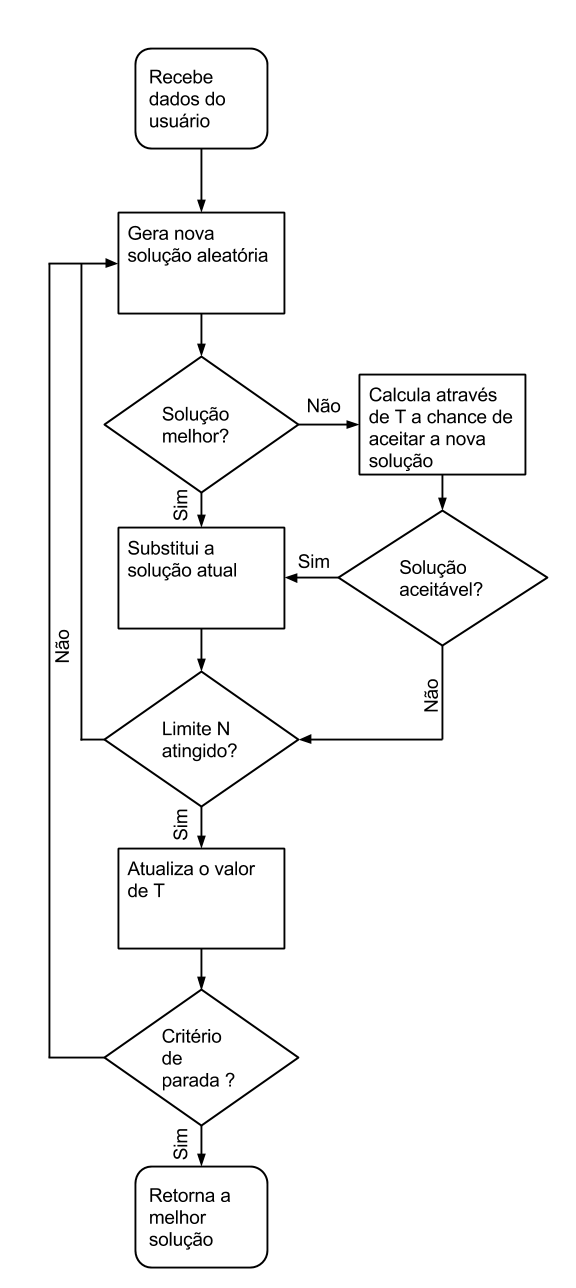
\includegraphics[scale=.5]{img/fluxsa.png}
\caption{Fluxograma do Método {\it Simulated Annealing}.} 
\label{fluxsa}
\end{figure}

{\it Simulated Annealing} (SA) é uma meta heurística genérica para problemas de otimização global que consiste em uma técnica de busca local probabilística. É usada normalmente em grandes espaços de busca e se fundamenta numa analogia com a segunda lei da termodinâmica. Seu nome é inspirado no processo de recozimento, utilizado em metalurgia para obtenção de estados de baixa energia num sólido. Neste processo, o metal é inicialmente aquecido à altas temperaturas e, em seguida, é resfriado lentamente e seu resfriamento é acompanhado e controlado de acordo com funções específicas. 

O método utiliza portanto um valor $T$ que é corresponde à temperatura, este valor é reduzido durante a execução. Inicialmente é gerada uma solução aleatória, sendo que em algumas implementações o valor $T$ pode ser usado como parâmetro de controle do componente aleatório. Nesse momento, a temperatura $T$ assume um valor elevado e, conforme o algoritmo progride, esse valor pode ser decrementado. 

Para cada nova solução gerada ocorre a comparação entre o resultado encontrado e a melhor solução encontrada. Se a solução encontrada for melhor que a anterior, esta é substituída pela nova solução. Caso contrário, ultiliza-se uma função (Equação \ref{anneq}) onde pode ser aplicado o Fator de Boltzmann, para determinar se a solução será aceita \cite{brooks1995optimization}. Nesta equação $kT$ é o Fator de Boltzmann e $E$ é a energia em um determinado estado.

\begin{equation}\label{anneq}
F({\rm aceitabilidade}) \propto e^{-\frac{E}{kT}}$$
\end{equation}

Como consequência, no início do processo, quando a temperatura é maior, é mais provável aceitar novas soluções, mesmo que inferiores em relação à função objetivo. Tal probabilidade diminui exponencialmente ao longo da execução. Através desta estratégia, o método SA tenta superar as barreiras energéticas e escapar de mínimos locais. 

Conforme ilustra o fluxograma da Figura \ref{fluxsa}, após um número $N$ determinado de novas soluções, o valor da temperatura $T$ é atualizado. Este processo se repete até que o critério de parada seja atingido. Esse critério pode ser um valor mínimo para a temperatura, um número fixo de etapas ou mesmo um tempo limite definido pelo usuário.

\section{Algoritmos de Distribuição Estimada}

Os Algoritmos de Distribuição Estimada (EDA) pertencem à classe de algoritmos evolutivos e também serviram de inspiração para a solução proposta nesse trabalho. Esses algoritmos já foram aplicados ao problema de dobramento apresentando bons resultados. 

\begin{figure}[htbp]
  \centering 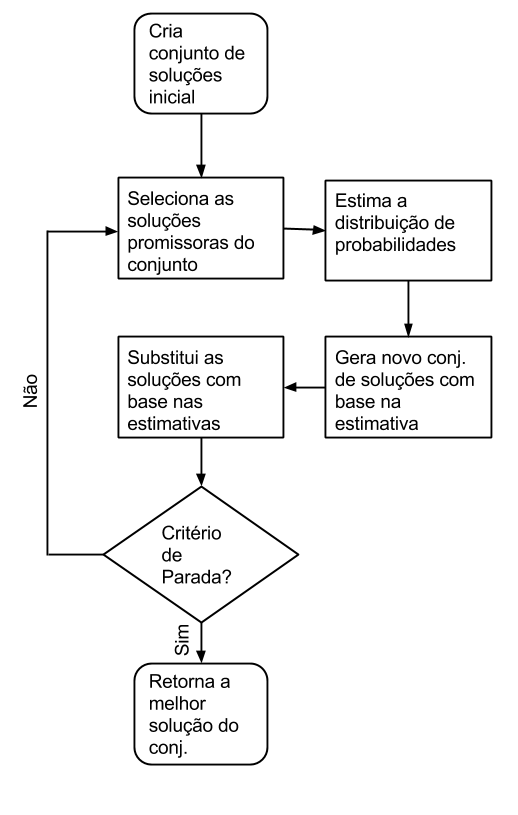
\includegraphics[scale=.55]{img/fluxeda.png}
\caption{Fluxograma de EDAs.} 
\label{fluxeda}
\end{figure}

A principal diferença entre EDAs e algoritmos evolutivos mais convencionais é que os algoritmos evolutivos geram novas soluções candidatas utilizando uma distribuição implícita definida por um ou mais operadores de variação, enquanto EDAs utilizam uma distribuição de probabilidade, que pode ser codificada por uma rede Bayesiana, uma distribuição normal multivariada, ou outra classe de modelo.

Conforme demonstra a Figura \ref{fluxeda}, os EDAs iniciam a busca criando um conjunto de soluções. De forma análoga, este conjunto seria denominado população em um algoritmo evolutivo. Inicia-se então um ciclo de análise dos resultados, seleção de bons resultados e geração de novo conjunto de soluções. O critério de parada que interrompe o ciclo pode ser de acordo com o número de etapas, o tempo de execução, entre outros.

Diversas técnicas são usadas para otimizar a busca desses algoritmos. É possível dividir os EDAs em classes de complexidade através da análise dos modelos probabilísticos usados por essas técnicas. 

Considerados mais simples algoritmos como PBIL ({\it Population-Based Incremental Learning}), cGA ({\it Compact Genetic Algorithm}), e UMDA ({\it Univariate Marginal Distribution Algorithm}) consideram todas as relações entre variáveis como independentes \cite{armananzas2008review}, fatorando o espaço de busca, considerando a probabilidade conjunta dos pontos como um produto de probabilidades marginais univariadas.

Algoritmos como MIMIC ({\it Mutual Information Maximization for Input Clustering}), BMDA ({\it Bivariate Marginal Distribution Algorithm}) e os baseados em árvores de depêndencia podem ser classificados como bivariados. Esses algoritmos podem representar as relações mais simples entre as variáveis e podem ser combinados para representar relações mais complexas.

Os EDAs multivariados fatorizam a distribuição de probabilidade das relações entre as conexões em uma ordem maior que dois. Dentre eles estão o BOA ({\it Bayesian Optimization Algorithm}), EcGA ({\it Extended compact Genetic Algorithm}) e o FDA ({\it Factorized Distribution Algorithm}), que usa um modelo fixo de interações em todas as gerações. Quanto maior a estrutura probabilística e o grau de complexidade da análise dos dados, maior o esforço computacional em encontrar as soluções que melhor se adaptam a essas funções.

Algumas implementações de EDA, assim como os algoritmos evolutivos têm dificuldade em encontrar a solução ótima para proteínas com sequências longas \cite{chen2009novel}. Essa dificuldade pode ser descrita como uma convergência prematura das soluções devido à falta de diversidade na sua geração. 

\section{Aprendizagem de Máquina}

O conceito de Aprendizagem de Máquina pode ser descrito como um processo que gira em torno de aprender através de uma determinada experiência \cite{anderson1986machine}. Um programa de computador é dito capaz de  aprender com a Experiência $E$ a respeito de uma classe de Tarefas $T$ com Performance $P$, se a performance nas mesmas tarefas $T$, melhora em relação à $P$ devido à experiência $E$. Ou seja, pode-se dizer que uma máquina aprende, se ela melhora sua performance na solução de um problema através da experiência acumulada nas soluções anteriores \cite{anderson1986machine}. 

A palavra “performance” pode ser analisada neste conceito como uma analogia ao desempenho da máquina, visto aqui como o rendimento na execução das Tarefas. Existe portanto, uma análise dos resultados da execução das tarefas $T$ em relação à requisitos ou metas. É importante observar que o conceito de melhoria na performance pode ser observado sob diferentes perspectivas. Uma primeira análise pode apontar para uma vantagem em relação ao tempo de execução, porém outros aspectos também são relevantes como a qualidade dos resultados. 

Os resultados das tarefas ou exemplos de treinamento têm uma distribuição de probabilidade de certa forma desconhecida. A máquina aprendiz tem que extrair deles algo mais geral, sobre a sua distribuição, que lhe permitirá produzir previsões úteis em novos casos.

Outra forma de analisar a aprendizagem é ver como seu objetivo determinar uma hipótese $H$, idêntica ao alvo conceito $C$, ao longo de todo um conjunto de instâncias $X$. A única informação disponível sobre $C$, nesse caso, é o seu valor ao longo dos exemplos de treinamento. Portanto, algoritmos de aprendizado indutivo, ou seja, algoritmos que utilizam um conjunto de dados de treinamento, podem, no máximo, garantir que a hipótese de saída se encaixa no conceito $C$ ao longo dos dados de treinamento. Na falta de mais informações, considera-se que o melhor hipótese sobre todos os casos, inclusive os não observáveis, é a hipótese que melhor se ajusta aos dados de treinamento observados. 

Uma máquina aprendiz que não faz suposições {\it a priori} sobre a identidade do conceito alvo não tem nenhuma base racional para a classificação das instâncias não observáveis, esta é uma propriedade fundamental da inferência indutiva \cite{anderson1986machine}. Devido à importância dos exemplos de treinamento para as técnicas de aprendizagem de máquina, podemos caracterizar essas técnicas de acordo com o o tipo de inferências indutiva realizada através desses exemplos. A idéia principal a ser percebida é a política através da qual a máquina aprendiz generaliza os dados não observáveis, para inferir a classificação de novas instâncias. Uma vantagem de visualizar esses sistemas de inferência em termos do viés indutivo é que ele fornece uma forma de caracterizar a sua política de generalização dos dados. Uma segunda vantagem é que permite a comparação dos diferentes aprendizes de acordo com sua capacidade indutiva. Para ilustrar essa idéia são analisadas algumas técnicas de aprendizagem de máquina \cite{anderson1986machine}. 

O algoritmo {\it Rote-Learner}, que aprende por repetição, simplesmente armazena os dados de treinamento em memória. As instâncias futuras são classificadas comparando-as com esses dados na memória. Se a instância é encontrada, ela recebe a mesma classificação armazenada em memória, do contrário o sistema não retorna nenhuma classificação. Este algoritmo não faz induções, toda classificação fornecida segue dedutivamente o que foi observado nos exemplos de treinamento.

Em um algoritmo de eliminação de candidatos, ({\it Candidate-Elimination Algorithm}) novas instâncias são classificadas somente se todos os membros classificadores da versão atual do espaço concordam com a classificação. Do contrário, o sistema se recusa a prover uma classificação. Neste caso existe um certo nível de indução, portanto este método classificará instâncias que o algoritmo {\it Rote-Learner} não seria capaz de classificar. 

O algoritmo denominado {\it Find-S} busca a hipótese mais específica que condiz com os exemplos de treinamento. A partir desta hipótese ele classifica todos as instâncias futuras. Este algoritmo tem um viés indutivo ainda maior, pois além de considerar que todas as instâncias podem ser classificadas através da hipótese específica, também supõe que o conceito alvo está contido neste espaço hipotético.

Quanto mais indutivo for o algoritmo de aprendizagem, maior a parcela de instâncias que ele será capaz de classificar. O nível de correção dessas classsificações depende obviamente da qualidade do método indutivo e dos exemplos de treinamento \cite{anderson1986machine}.

\chapter{Trabalhos relacionados}

Neste capítulo são discutidos trabalhos relacionados ao algoritmo proposto nessa dissertação. São discutidos trabalhos que apresentam algoritmos para predição de proteínas reais e principalmente trabalhos que implementam algoritmos de dobramento considerando o Modelo AB. São destacados os trabalhos que foram utilizados no Capítulo 5 onde é apresentada a comparação dos resultados obtidos com o algoritmo proposto com os trabalhos relacionados. 

Conforme explicado, predizer a estrutura nativa de uma proteína a partir de sua sequência é um dos problemas mais difíceis em Bioinformática. Esta dificuldade provem de dois aspectos: o tamanho do sistema é da mesma ordem do número de átomos envolvidos e o espaço de soluções é, por consequência, muito complexo. Este espaço de soluções pode ser descrito como uma série de mínimos locais, separados por barreiras com altíssimos valores energéticos.

Anfisen \cite{anfinsen1972studies} analisa detalhadamente o dobramento de proteínas reais a partir de uma série de aspectos do problema, como as relações não locais e a conformação de núcleos e padrões locais. Porém, mesmo percebendo a complexidade do problema, considera que com a crescente quantidade de dados disponível e com a evolução teórica, a ideia de prever o dobramento de proteínas tem se tornado mais realista. De acordo com a hipótese de Anfisen \cite{anfinsen1973principles}, a estrutura terciária nativa de uma proteína pode ser determinada a partir da informação contida na sequência primária, o que permitiria que métodos computacionais fossem desenvolvidos para predizer estruturas terciárias quando a primária estivesse disponível. 

Considerando que a configuração que possui menor energia livre é a conformação nativa da proteína-alvo, essa hipótese levanta dois principais problemas. O primeiro é desenvolver uma fórmula que defina a energia de uma proteína real. O segundo problema é desenvolver os métodos computacionais de otimização para busca da energia mínima através dessa fórmula. No entanto, ainda não existem ferramentas computacionais capazes de predizer a estrutura tridimensional de uma grande variedade de proteínas. Devido à complexidade do problema modelos simplificados foram propostos.

O modelo simplificado mais utilizado é conhecido como Modelo HP (Lattice), onde cada aminoácido é tratado como um vértice de uma grade ortogonal de duas ou três dimensões \cite{dill1985theory}. Neste modelo simplificado, as sequências são compostas por dois tipo de aminoácidos: $H$ hidrofóbicos e $P$ hidrófilos. Sendo o modelo mais simplificado, somente as interações não conectadas nos resíduos tipo $H$ vizinhos são consideradas, negligenciando outras relações não locais causadas por ligações $P$-$P$, $H$-$P$ e $H$-$H$ não vizinhos. 

Em um artigo sobre o dobramento de proteínas, Unger e Moult \cite{unger1993genetic} descrevem um Algoritmo Genético que utiliza cruzamento baseado em heurísticas e operadores de mutação para resolver o Modelo HP. O algotimo genético foi capaz de superar os métodos de Monte Carlo (MC) \cite{stillinger1995collective} em diferentes sequências. É importante salientar que os algoritmos propostos para solucionar o Modelo HP podem não ser extensíveis ao Modelo AB devido ao formato das soluções não discreto do Modelo AB. E, mesmo naqueles em que é possível uma adaptação, pode resultar em uma grande perda de eficiência.

Conforme decrito na Seção 2.8, EDAs são algoritmos evolutivos que constroem um modelo probabilístico explícito a partir de um conjunto de soluções selecionadas. Desta forma, pode-se captar interações relevantes entre as variáveis do problema, analisando prováveis dependências existentes. Um algoritmo de estimação de distribuição utilizando o modelo de Markov \cite{santana2008protein} apresentou resultados ainda melhores que os de outros métodos baseados em populações ou conjuntos de soluções no Modelo HP.

Em 1993, Stillinger, Head-Gordon e Hirshfeld publicaram um modelo de proteínas simplificado que considerava os efeitos não locais e iniciaram os estudos desse modelo através de algoritmos baseados em redes neurais. Nesse artigo \cite{stillinger1993toy}, são analisadas trímeros, tetrâmeros e pentâmeros, e é apresentada uma tabela com as conformações de menor energia para todas estas sequencias de aminoácidos.

A partir da análise apresentada neste artigo \cite{stillinger1993toy} é possível perceber que algumas sequencias de aminoácidos deste modelo apresentam como conformação mais estável, ou seja, de menor energia, uma proteína linear. Estes casos não são relevantes para o problema de dobramento pois o objetivo do modelo é encontrar conformações similares às encontradas na natureza. Na Tabela \ref{tabelastill} são apresentados os resultados relevantes para este trabalho obtidos por Stillinger.

\begin{table}
\begin{center}
\caption{Resultados obtidos por Stillinger \cite{stillinger1993toy}}\label{tabelastill}
\begin{tabular}{lr}
\hline
Cadeia & Energia \\
\hline
FIBO3(BAB) & -0.3027\\
TETRA0(AAAA) & -1.67633\\
TETRA1(AAAB) & -0.58527\\
TETRA2(AABA) & -1.45098\\
TETRA3(AABB) & 0.06720\\
TETRA4(ABAB) & -0.64938\\
TETRA5(ABBA) & -0.03617\\
TETRA6(ABBB) & 0.00470\\
TETRA7(BAAB) & 0.06172\\
TETRA8(BABB) & -0.00078\\
TETRA9(BBBB) & -0.13974\\
FIBO5(ABBAB) & -0.00565\\
\hline
\end{tabular}
\end{center}
\end{table}

Em um artigo posterior, Stillinger \cite{stillinger1995collective} ressalta a importância das sequências de aminoácidos para o Modelo AB e são analisadas diferentes sequências para proteínas maiores, de até 55 aminoácidos. Dois tipos de sequências são analisadas, o primeiro tipo é denominado {\it Center Doped} e usa o padrão ($An$-$B$-$An$), enquanto o segundo se inspira na série de Fibonacci. As proteínas geradas a partir de sequencias de Fibonacci apresentaram características muito relevantes como a conformação de padrões locais e soluções distintas para diferentes  polímeros, por isso este trabalho utiliza este sequenciamento. Stillinger \cite{stillinger1995collective} reafirma ainda a imensa dificuldade computacional intrínseca em prever o dobramento de grandes proteínas. 

O artigo em que apresenta o Modelo AB \cite{stillinger1993toy}, utiliza algoritmos de Redes Neurais para obter seus resultados de dobramento. Também conhecidos como Redes Neurais Artificiais, são algoritmos que simulam os neurônios no seu funcionamento e são muito eficientes em métodos de classificação.

Outras formas de explorar o problema de dobramento de proteínas com o Modelo AB já utilizadas são baseadas no Método de Monte Carlo (MC) \cite{stillinger1995collective}. Este método também foi explorado por Stillinger e consiste em gerar amostragens aleatórias para obter resultados numéricos que representem o espaço de busca. Este método é muito comumente utilizado quando a distribuição probabilistica do espaço de busca é desconhecida, como é o caso do problema de dobramento. Dentre essas técnicas, a que apresentou resultados mais relevantes é denominada Annealing Contour Monte Carlo (ACMC) \cite{liang2004annealing}.

ACMC é uma versão acelerada do algoritmo CMC ({\it Countour Mounte Carlo}) para problemas de dobramento.
O CMC é uma generalização do algoritmo {\it Wang-Landau} e do algoritmo  1/$k$-{\it ensemble} e pode ser utilizado em sistemas discretos e contínuos. Devido à capacidade de auto ajuste, o CMC é capaz de superar qualquer barreira energética no espaço de busca. O ACMC propõe uma divisão desse espaço de busca em regiões, sendo que o número de regiões diminue ao longo da busca através de uma função específica \cite{liang2004annealing}. 

Após a proposta do Modelo AB, diversos estudos foram realizados com diferentes algoritmos, como {\it Conventional Metropolis Monte Carlo} e {\it Simulated Tempering} \cite{irback1997local}. Entre as técnicas que merecem destaque no campo do dobramento: {\it Multicanonical Monte Carlo, Pruned-Enriched Rosenbluth Method} \cite{hsu2003structure}, {\it Simulated Tempering} e {\it Artificial Bee Colony} \cite{li2014protein} . 

Neste trabalho é apresentado, no Capítulo 5, um conjunto de resultados onde as soluções de dobramento para diferentes sequências são comparadas entre o algoritmo proposto e alguns trabalhos relacionados que merecem destaque como o algoritmo CSA ou {\it Conformational Space Annealing}. O método CSA busca todo o espaço de soluções em seus estágios iniciais, depois estreita a busca para regiões menores de baixa energia de acordo com uma distância determinada \cite{lee2008re}. 

Outro algoritmo que serve de comparação nos resultados é o {\it Statistical Temperature Molecular Dynamics} (STMD). Este método se diferencia por utilizar dados estatísticos relacionados à temperatura no lugar das densidades dos estados em uma distribuição {\it Wang-Landau}. O trabalho comparado \cite{kim2006statistical} que utiliza esse algoritmo também apresenta implementação e resultados para o Modelo AB tridimensional.

O algoritmo {\it Heuristic-based Tabu Search} (HTS) têm sido aplicado com sucesso em problemas de otimização \cite{liu2013heuristic}. Integrando mecanismos de conformação heurística e o método tradicional {\it Tabu Search} (TS), o algoritmo apresentou bons resultados para o Modelo AB e também aparece na tabela de comparações de resultados desse trabalho.

A Tabela \ref{tabelarela} relaciona os trabalhos que serão utilizados como comparação e demonstra quais as sequências utilizadas em cada um deles. Todos algoritmos apresentados neste artigo compartilham do mesmo desafio: Ultrapassar as barreiras energéticas do espaço de soluções e escapar dos ótimos locais para atingir a real solução do problema. 

\begin{table}
\begin{center}
\caption{Comparação dos trabalhos relacionados}\label{tabelarela}
\begin{tabular}{lccccr}
\hline
Algoritmo & Seq. de Fibonacci & Proteínas reais & Modelo AB 3D\\
\hline
ACMC \cite{liang2004annealing} & 13 - 55 & Não & Sim\\
STMD \cite{kim2006statistical} & 55 & Não & Sim\\
HTS \cite{liu2013heuristic} & 13 - 55 & Sim & Não\\
CSA \cite{lee2008re} & 13 - 55 & Não & Sim\\
ELA+ANN (Proposta) & 13 - 55 & Sim & Não\\
\hline
\end{tabular}
\end{center}
\end{table}

A seguir é apresentada a proposta que tem como objetivo superar essas barreiras através de métodos inspirados em {\it Simulated Annealing}, aprendizagem de máquina e EDAs e buscam utilizar a distribuição de probabilidade para extrair dados que auxiliem na evolução da busca pela solução.

\chapter{Proposta de algoritmo para o Modelo AB}

Neste trabalho são propostos dois algoritmos para dobramento de proteínas no Modelo AB. O primeiro algoritmo, chamado de algoritmo ANN é inspirado no {\it Simulated Annealing}. Esse algoritmo utiliza uma variável para gerar novas soluções cujo valor diminui ao longo da sua execução. Nesse algoritmo, a busca pela solução não utiliza nenhum tipo de aleatoriedade. Devido à sua simplicidade, este método converge sempre para um ótimo local. 

Por esse motivo foi desenvolvido um algoritmo mais complexo denominado ELA, capaz de explorar o espaço de busca de forma inteligente. O segundo algoritmo proposto é baseado nos algoritmos EDAs e nos conceitos de aprendizagem de máquina e utiliza dois parâmetros básicos para gerar novas soluções: Rigidez e Eficiência. Os valores desses parâmetros são ajustados de acordo com a busca e têm como objetivo representar a distribuição de probabilidade das instâncias não observáveis.

Os dois algoritmos são utilizados em conjunto, sendo primeiramente aplicado o algoritmo ELA para realizar uma busca inicial, gerando novas soluções, aplicando em seguida o algoritmo ANN para refinar as melhores soluções encontradas. Foi desenvolvida então uma aplicação para realizar a execução os algoritmos na ordem desejada. Essa aplicação também cumpre a função de serializar os testes, gerar dados para análise e desenvolvimento e exibir as soluções graficamente. 

\section{Algoritmo ANN}

De forma análoga ao método {\it Simulated Annealing}, porém de forma simplificada, foi desenvolvido o algoritmo ANN que substitui a solução atual por uma solução próxima, escolhida de acordo com uma função objetivo e com uma variável que representa a temperatura ou a quantidade de energia da busca. 

À medida que o algoritmo progride, o valor dessa variável é decrementado, dessa forma a busca gera valores menores, convergindo a solução para um ótimo local. No problema de dobramento essa variável com o valor inicialmente alto representa o ângulo entre os aminoácidos e a função objetivo é a Equação \ref{energyeq} apresentada na Seção 2.4.

\begin{figure}[htbp]
  \centering 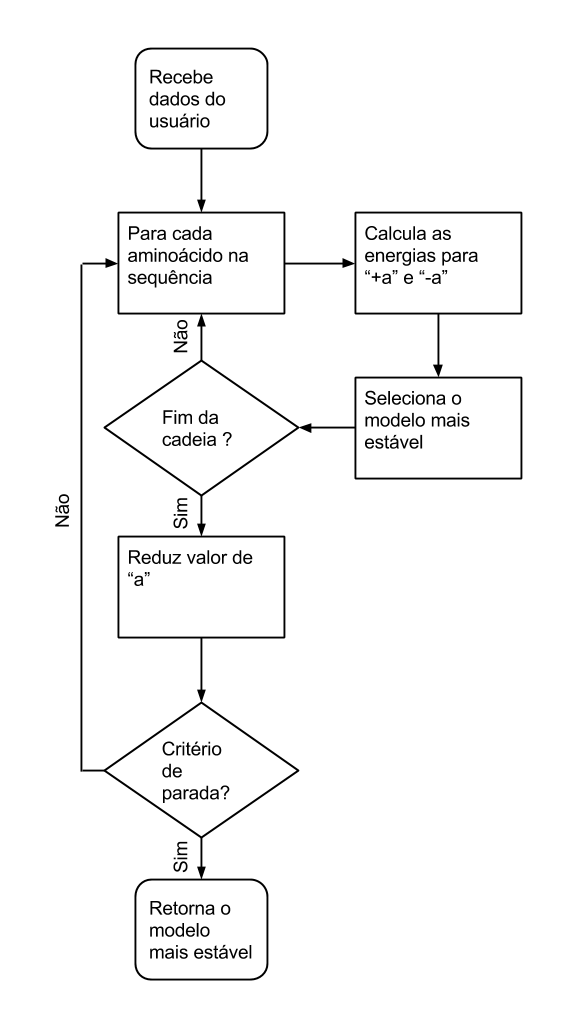
\includegraphics[scale=.55]{img/fluxann.png}
\caption{Fluxograma do algoritmo ANN inspirado em {\it Simulated Annealing}.} 
\label{fluxann}
\end{figure}

\begin{algorithm}
  \caption{Pseudo código do algoritmo ANN inspirado em {\it Simulated Annealing}}\label{annalg}
  \begin{algorithmic}
 
  \WHILE{stopCriteria}
   \FOR{amino in protein}
     \STATE{esq = amino.ang + a}
     \IF{esq < min} 
       \STATE{min = esq}
     \ENDIF
     \STATE{dir = amino.ang - a}
     \IF{dir < min} 
       \STATE{min = dir}
     \ENDIF
    \ENDFOR
    \STATE{a = a * delta}
  \ENDWHILE
  \STATE{\RETURN min}
  
  \end{algorithmic}
\end{algorithm}

\begin{figure}[htbp]
  \centering 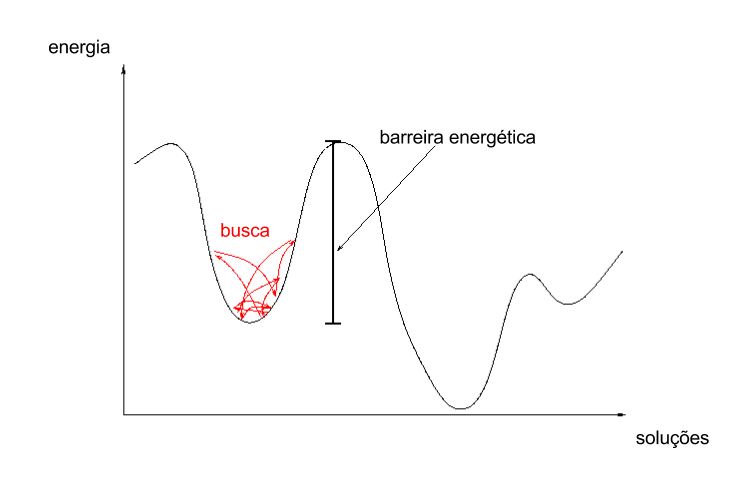
\includegraphics[scale=.46]{img/barreira.png}
\caption{Busca restrita à uma região com soluções não ótimas.} 
\label{barreira}
\end{figure}

Esse algoritmo não possui nenhuma função específica que torne possível a aceitação de soluções inferiores às encontradas anteriormente e não utiliza nenhum tipo de aleatoriedade. Devido ao fato de o algoritmo não apresentar ferramentas para escapar de situações em que a conformação apresenta um valor de energia baixo em relação às conformações vizinhas (ótimos locais), a busca não parte para uma conformação inicial promissora. 

O funcionamento do algoritmo ANN está resumido no fluxograma apresentado na Figura \ref{fluxann}. Este algoritmo pode ser descrito como uma versão simplificada do método {\it Simulated Annealing} tradicional e funciona da seguinte forma: o valor inicial $a$ dos ângulos é determinado pelo usuário. A cada etapa, cada ângulo do modelo é alterado nas duas direções, positiva e negativa, calculando a energia de ambas conformações. É escolhida então a conformação mais estável entre as três conformações calculadas (direção positiva +$a$, direção negativa -$a$ e não alterar o ângulo). Após o cálculo do último ângulo da cadeia é decrementado o valor de $a$ através do parâmetro $delta$. 

O parâmetro $delta$ é definido entre 0 e 1 e determina como será reduzida a temperatura, conforme demonstra o Algoritmo \ref{annalg}. O valor $a$ é multiplicado por $delta$, dessa forma o ângulo $a$ tende a 0 ao longo da execução. Caso o critério de parada definido pelo usuário não tenha sido atingido, inicia-se então uma nova execução.

Apesar do algoritmo ANN não apresentar bons resultados no início da busca por uma solução, se mostrou um bom método para refinar soluções. O algoritmo fica restrito à áreas cujo perímetro é formado por soluções com alto valor energético, em outra palavras, ele não ultrapassa as barreiras energéticas (Figura \ref{barreira}) entre os ótimos locais. Porém o algoritmo se demonstrou muito eficaz como método de descida, ou seja, em finalizar buscas, ajustando os ângulos até a melhor conformação local.

Dessa forma, optou-se por executar esse algoritmo para refinar a solução encontrada por outro método capaz de explorar o espaço de busca de forma inteligente, sem retringir-se a esses “vales”, ou ótimos locais, que impedem o caminho para a solução ótima. 

Por esse motivo, neste trabalho foi desenvolvido um novo algoritmo, com o objetivo de melhorar a busca por dobramentos iniciais, considerando a problemática dos ótimos locais. Esse algoritmo chamado de ELA foi desenvolvido para atuar em conjunto com o ANN e é descrito na próxima seção. 

\section{Algoritmo inspirado em Distribuição Estimada - ELA}

De forma a contornar os problemas apresentados pelo algoritmo ANN, foi desenvolvida uma solução que utilizasse técnicas menos diretas, que tratassem o problema em um nível mais subjetivo. Buscou-se então, conceitos mais abrangentes, que pudessem ser aplicados à diversas classes de problemas. Dentre esses conceitos, dois foram os que serviram de inspiração para esta proposta: o conceito de  Aprendizagem de Máquina (Machine Learning) e os algoritmos de Distribuição Estimada (EDAs).

O conceito de aprendizagem de máquina foi incorporado ao algoritmo ELA proposto neste trabalho para o dobramento de proteínas de forma que, a cada dobramento, um conjunto de dados ou parâmetros proveniente da busca pela solução fosse armazenado. Essa a memória onde ficam armazenados os valores dos parâmetros, guarda a experiência do algoritmo. Ao gerar novos dobramentos o algoritmo usa os parâmetros para obter melhores soluções. Através desta heurística, os parâmetros se adaptam na medida que a busca prossegue, de forma a direcionar a geração de novas soluções. 

A inspiração proveniente dos EDAs para o algoritmo proposto foi a de utilizar fatores de aleatoriedade sempre guiados explicitamente por valores específicos. Esses valores são extraídos da própria solução do problema e por isso moldam probabilisticamente o caminho para a solução. A partir desses conceitos, foi desenvolvido o algoritmo, denominado Algoritmo de Aprendizagem Estimada ({\it Estimated Learning Algorithm} - ELA), onde esses valores são usados para selecionar e gerar ângulos. 

O algoritmo ELA proposto parte de uma proteína no Modelo AB com sua sequência de aminoácidos linear e por meio de dois parâmetros, chamados de Rigidez e Eficiência, ajusta os ângulos entre os aminoácidos sucessivamente. Após cada ajuste, ou dobras, a energia da proteína é calculada e os parâmetros são atualizados com base nos resultados. 

O pseudo código descrito no Algoritmo \ref{elaalg} e no fluxograma da Figura \ref{fluxela} resume o funcionamento do algoritmo. Inicialmente é gerado um conjunto de soluções inicial, ou população, totalmente formado por soluções lineares. Em seguida são inicializados os parâmetros de Rigidez e Eficiência, cada um com o mesmo comprimento da cadeia menos dois (o primeiro e o último ângulo não são relevantes). 

A partir daí, a cada etapa, são selecionados os primeiros resultados que servirão de referência para a geração de novas soluções. Em seguida, para cada item do conjunto de soluções é feita uma seleção aleatória multinomial através da Eficiência para definir quais ângulos serão alterados. É então realizada a alteração dos ângulos aleatoriamente através de uma função Gaussiana que considera a Rigidez. Por fim, o conjunto de soluções é ordenado por energia de forma crescente, sendo o modelo mais estável o primeiro do conjunto. Caso o critério de parada definido pelo usuário não tenha sido atingido, inicia-se uma nova etapa, caso contrário, o algoritmo retorna o primero item do conjunto.

O número de resultados utilizados para a geração de novas soluções é calculado através de um parâmetro ($parent$) que define a porcentagem do conjunto de soluções que será utilizada. 

\begin{algorithm}
  \caption{Pseudo código do algoritmo ELA inspirado em EDA}\label{elaalg}
  \begin{algorithmic}
  \FOR{p in population}
       \STATE{population[p] = new Protein([ang: linear, a - 2])}
  \ENDFOR
  \FOR{a in protein}
    \STATE{parameters = initParameters([efficiency: [1, a - 2], rigidity: [1, a - 2]])}
  \ENDFOR
  \WHILE{stopCriteria}
    \FOR{p in population}
      \STATE{ref = population[ int(p * parent) ]}
    \ENDFOR
    \STATE{sum = 0}
    \FOR{a in parameters}
      \STATE{parameters[a].low = sum}
      \STATE{sum = sum + parameters[a].efficiency}
      \STATE{parameters[a].up = sum}
    \ENDFOR
    \STATE{r = random * sum}
    \FOR{a in parameters}
      \IF{parameters[a].low <= r and r < parameters[a].up}
        \STATE{selectedAngle.push(a)}
        \STATE{parameters[a].remove()}
      \ENDIF
    \ENDFOR
    \STATE{p = [ang: gaussRandom(selectedAngle[a], 1/rigidity)\%(PI*2)]}
    \STATE{population.push(new Protein(p))}
    \STATE{population.sortByEnergy()}\\
  \ENDWHILE
  \STATE{\RETURN population[0]}\\
  \end{algorithmic}
\end{algorithm}

O conceito denominado Eficiência ($efficiency$) representa a performance do dobramento de determinado aminoácido. Esse parâmetro é utilizado no momento em que é selecionado o ângulo onde serão realizadas as novas dobras. Esta seleção é aleatória e multinomial, sendo que quanto maior a Eficiência de um aminoácido do modelo, maior a chance dele ser selecionado conforme demonstrado na Figura \ref{eficiencia}. A Eficiência de um aminoácido pode aumentar quando a dobra realizada aumenta a estabilidade da proteína, assim o algoritmo aumenta as chances de sucesso das dobras seguintes. 

No exemplo da Figura \ref{eficiencia}, o quarto ângulo possui Eficiência igual a 4, o que implica em uma chance de 50\% de ser escolhido, enquanto os ângulos cuja Eficiência é igual a 1 têm somente 12,5\%.

A Eficiência é inicializada com valor um para todos os aminoácidos sendo este o valor mínimo aceitável, isso significa que, no início da execução, todos aminoácidos têm a mesma chance de serem selecionados. O limite máximo para os valores de Eficiência é determinado pelo usuário. Existem dois parâmetros que determinam como serão alterados os valores de Eficiência. Um parâmetro para os casos de sucesso, quando a solução encontrada é mais estável que aquela utilizada como referência. E outro parâmetro para os casos onde a energia encontrada é superior, ou seja, os casos de falha.

\begin{figure}[htbp]
  \centering 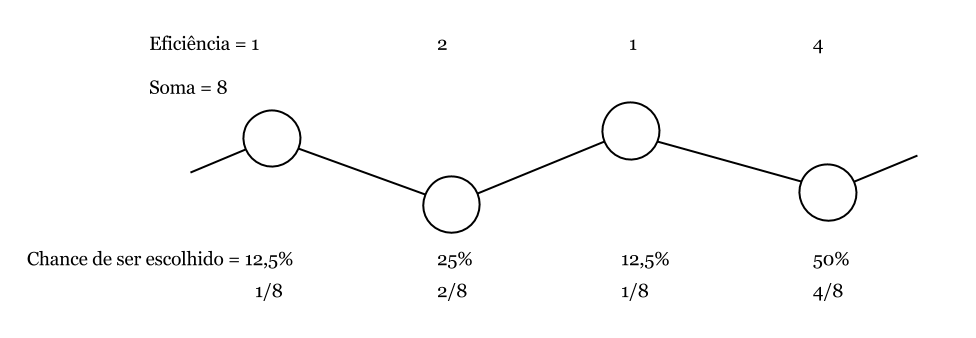
\includegraphics[scale=.45]{img/eficiencia.png}
\caption{Eficiência - Seleção de novos ângulos.} 
\label{eficiencia}
\end{figure}

A cada passo, são alterados um número determinado de ângulos ao longo da estrutura primária. Este número de ângulos estabelece uma relação de proporcionalidade com o comprimento da cadeia. Na situação onde se alteram muitos ângulos, a informação que relaciona quais destes ângulos contribuiu para a solução se torna menos confiável. Porém alterando somente um ângulo por vez, torna-se impossível encontrar o dobramento ótimo sem aceitar soluções energéticamente superiores, principalmente em proteínas com grandes cadeias primárias. Isso se deve ao fato de que, ao alterar somente um ângulo, estamos explorando uma única dimensão do espaço de soluções. O fato que não há um caminho constituído por linhas ortogonais que leve à solução ótima sem passar por soluções altamente instavéis é visível e está demonstrado na Figura \ref{orto}. Nos testes foi utilizado um número fixo de dois ângulos alterados por vez, este número foi selecionado com base na calibragem realizada para as sequências estudadas.

\begin{figure}[htbp]
  \centering 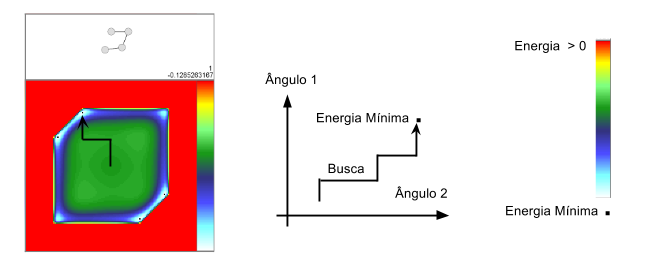
\includegraphics[scale=.6]{img/orto.png}
\caption{Busca alterando apenas um ângulo.} 
\label{orto}
\end{figure}

A Rigidez ($rigidity$) influencia diretamente no valor do incremento do ângulo gerado em cada novo dobramento, sendo que quanto mais rígido, ou seja quanto maior o valor do parâmetro do aminoácido que representa a Rigidez, menor provavelmente será o novo ângulo gerado. Dessa forma, no início da busca as mudanças são maiores (Figura \ref{rigidez} - Rigidez 1) e, na medida em que a proteína se dobra em estados mais estáveis, a Rigidez aumenta e também aumenta a probabilidade de gerar ângulos mais agudos, provocando assim um ajuste cada vez mais fino dos ângulos (Figura \ref{rigidez} - Rigidez 5). 

A Rigidez é inicializada com valor um para todos os aminoácidos sendo este o valor mínimo aceitável se e seu valor máximo é determinado pelo usuário. Utiliza-se uma função Gaussiana que considera o inverso da Rigidez como variância e o próprio valor do ângulo como média para gerar os valores dos novos ângulos. Em $Javascript$, esta distribuição normal foi implementada através do método polar \cite{sheldon2002first} .

\begin{figure}[htbp]
  \centering 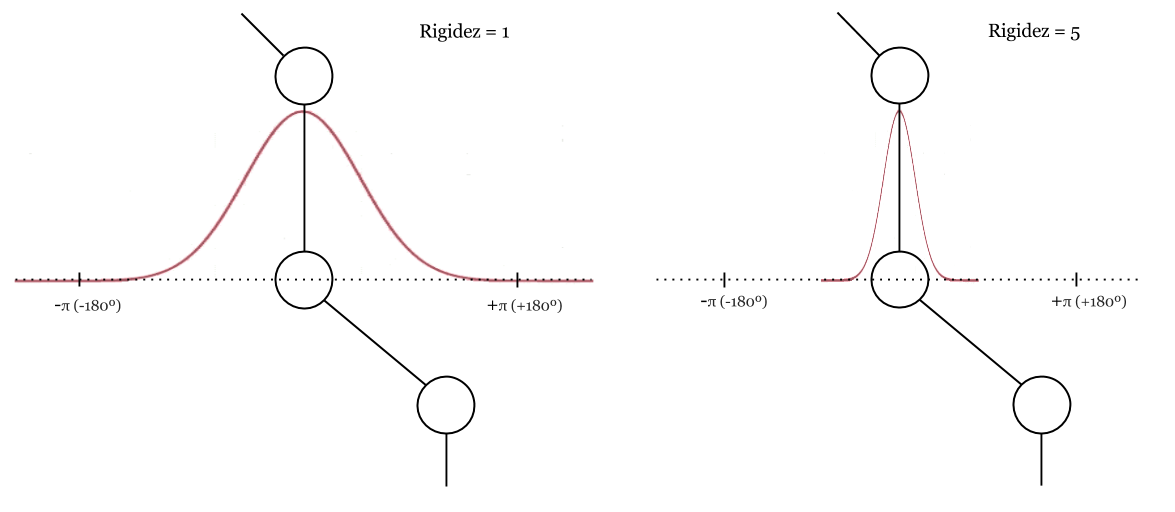
\includegraphics[scale=.35]{img/rigidez.png}
\caption{Rigidez - Geração de novos ângulos.} 
\label{rigidez}
\end{figure}

Os valores de Rigidez são alterados de forma similar aos valores de Eficiência. Existem dois parâmetros que ajustam os valores em caso de sucesso ou falha. Porém através de parâmetros específicos é possível alterar o valor da Rigidez dos ângulos vizinhos sempre que existe uma alteração dos parâmetros. Com isso é possível tornar uma determinada parcela da cadeia mais rígida, conservando assim trechos onde a dobra foi bem sucedida. Existem dois parâmetros que controlam este comportamento, um que determina o número de vizinhos afetados e outro que, através de uma expressão, altera o quanto os vizinhos especificados são afetados. 

\begin{figure}[htbp]
  \centering 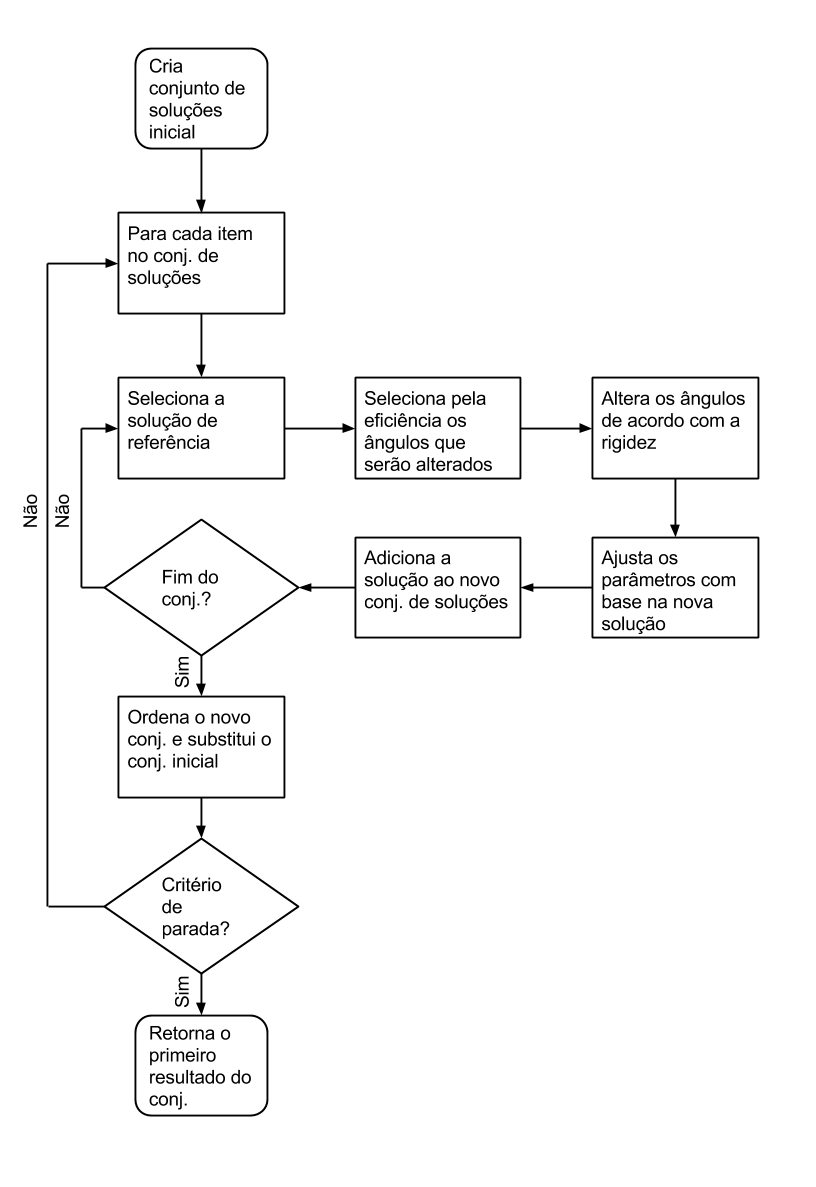
\includegraphics[scale=.5]{img/fluxela.png}
\caption{Fluxograma do algoritmo ELA inspirado em EDAs.} 
\label{fluxela}
\end{figure}

Após a geração de um conjunto de soluções com base nos parâmetros de Eficiência e Rigidez, este conjunto é ordenado com base no valor energético calculado através da Equação \ref{energyeq}. O algoritmo de ordenação utilizado pode variar de acordo com o comprimento da cadeia primária e é determinado pelo interpretador $Javascript$. O critério de parada do algoritmo é um parâmetro fixo informado pelo usuário. Esse parâmetro determina o número de etapas, sendo cada etapa definida como a geração, análise, ordenação e seleção de uma população ou conjunto de soluções.

\section{Aplicação para execução de experimentos}

Com o objetivo de serializar a execução dos algoritmos ANN e ELA, auxiliar a calibragem dos parâmetros e demonstrar os resultados obtidos, foi desenvolvida uma aplicação com interface de usuário amigável capaz de serializar os testes e armazenar os dados em disco para posterior análise. A aplicação recebe uma série de parâmetros inseridos pelo usuário e utiliza-os para realizar testes em série. Esta interface foi desenvolvida de forma a ser utilizada em paralelo à execução dos algoritmos, dando liberdade de análise e manipulação dos dados durante sua execução sem alterar sua performance.

A aplicação para execução dos experimentos envia os valores dos parâmetros para os algoritmos e recebe os resultados por meio dessa interface com o usuário. Entre estes parâmetros estão os valores limites para os algoritmos (critérios de parada), o comprimento do conjunto de soluções (tamanho da população), os valores que alteram a Eficiência e a Rigidez e seus limites, número de ângulos alterados por etapa, número de vizinhos alterados pela Rigidez, entre outros (Figura \ref{printapp}).

A aplicação executa os algoritmos em paralelo ao navegador, porém é importante ressaltar que somente um algoritmo é executado por vez, ou seja, somente a interface de usuário (User Interface - UI) funciona de forma paralela ao restante da aplicação. O único objetivo de excutar a UI em paralelo aos algoritmos é o de permitir que o usuário possa visualizar e editar os dados dos testes finalizados durante a execução de novos testes.

\begin{figure}[htbp]
  \centering 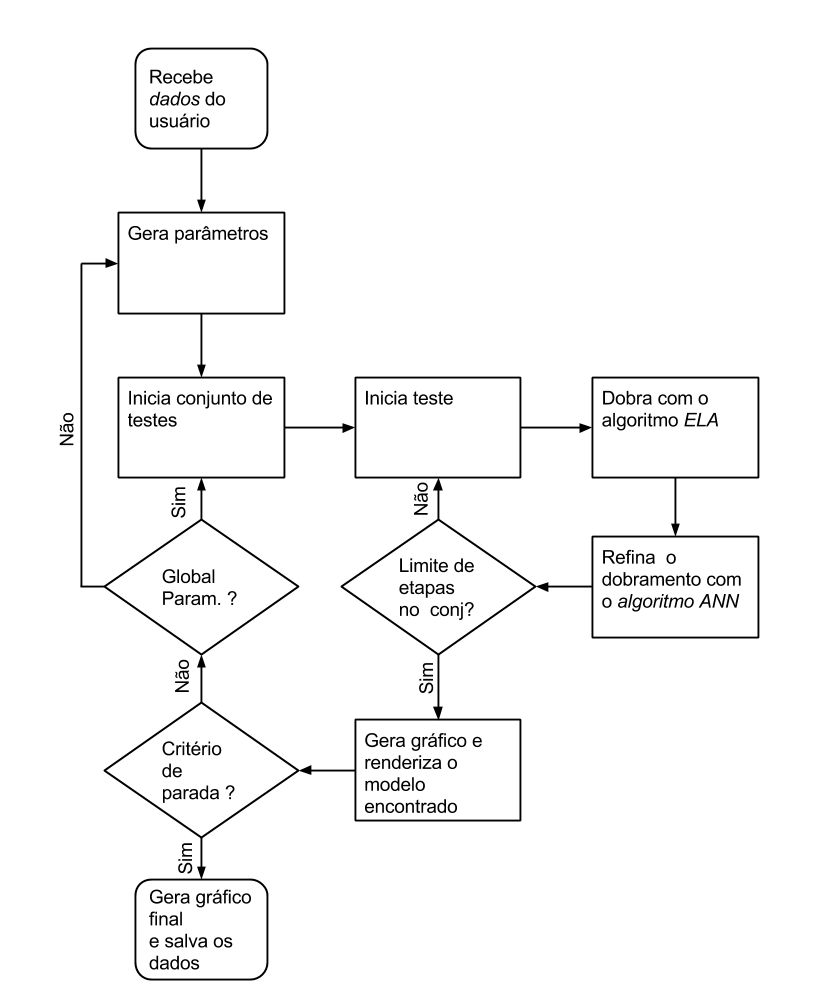
\includegraphics[scale=.55]{img/fluxapp.png}
\caption{Fluxograma da aplicação web.} 
\label{fluxapp}
\end{figure}

O funcionamento da aplicação está resumido no fluxograma da Figura \ref{fluxapp}. Após receber os dados iniciais, a aplicação inicializa  os parâmetros de Rigidez e Eficiência para o algoritmo ELA. Em seguida iniciam-se os testes sempre aplicando consecutivamente, por um número determinado de etapas, o algoritmo ELA seguido do algoritmo ANN. Os testes são divididos em conjuntos, com o objetivo de utilizar diferentes parâmetros para cada conjunto. Os conjuntos são necessários devido aos fatores aleatórios, sendo que a aplicação calcula a média dos testes dos conjuntos para análise.

A aplicação gerencia os parâmetros de Rigidez e Eficiência de modo a permitir que o usuário escolha se esses valores serão guardados após cada teste ou se haverá a reinicialização dos parâmetros a cada teste. Dessa forma, é possível observar como esses parâmetros se comportam após uma número específico de testes. 

\begin{figure}[htbp]
  \centering 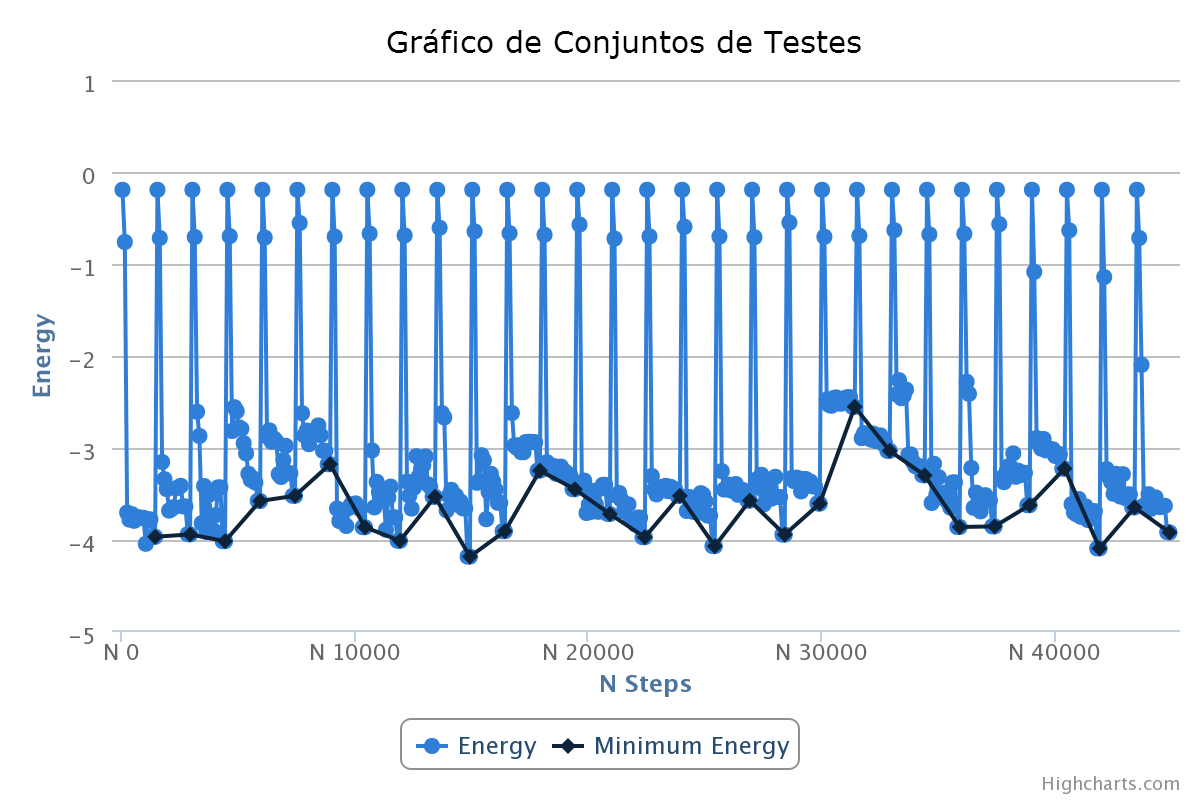
\includegraphics[scale=.3]{img/testchart.png}
\caption{Resultado gráfico de um conjunto de testes.} 
\label{testchart}
\end{figure}

Cada conjunto de testes é realizado repetidamente com os mesmos parâmetros para a mesma cadeia por um número de vezes previamente determinado. Uma tabela é preenchida em tempo real com os ângulos e energias do melhor modelo encontrado em cada teste. Ao fim de cada conjunto de testes, um gráfico (Figura \ref{testchart} ) é gerado demonstrando a performance dos modelos gerados.

\begin{figure}[htbp]
  \centering 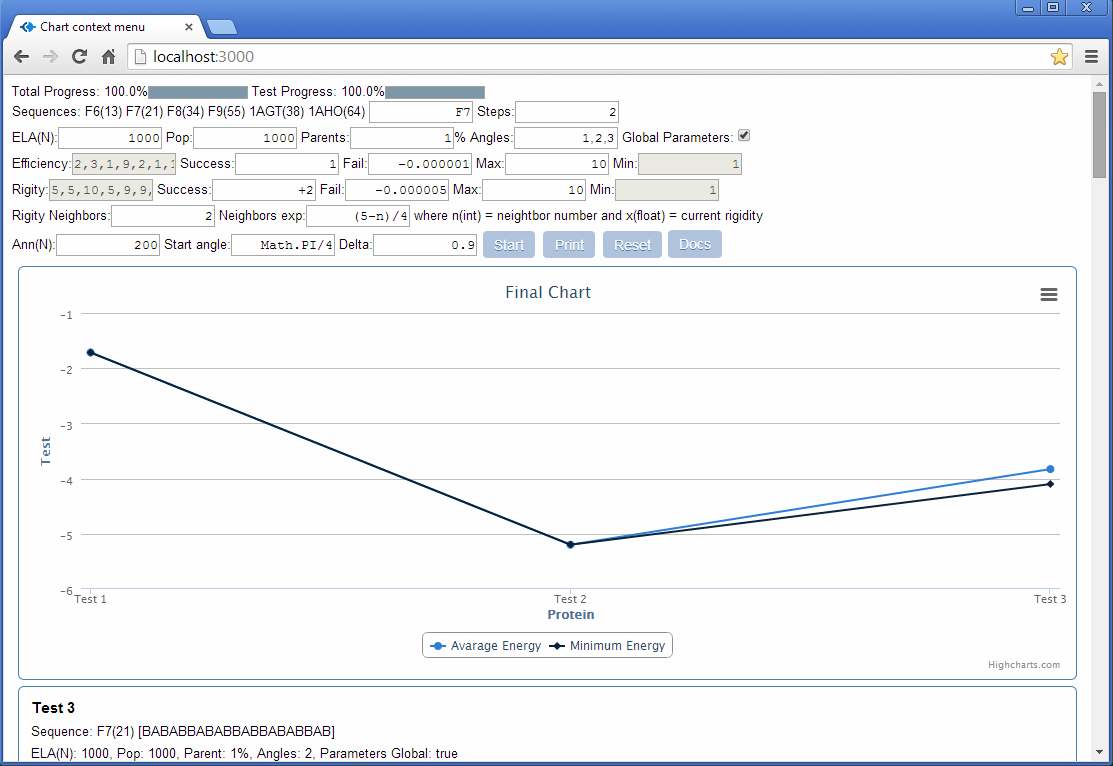
\includegraphics[scale=.4]{img/printapp.png}
\caption{Interface da aplicação para execução de experimentos.} 
\label{printapp}
\end{figure}

Desta forma é possível determinar se aquele conjunto de testes teve resultados semelhantes, ou se somente poucos modelos obtiveram valores energéticos pequenos. Para facilitar esta análise, ao fim da execução dos testes também é apresentada a média das energias de todos os testes. Também são exibidos o tempo médio e o tempo total de execução para cada modelo. O modelo mais estável é renderizado graficamente de forma a facilitar a análise visual da qualidade das dobras. 

A interface apresenta duas barras de progresso, sendo a segunda barra responsável por exibir em porcentagem o progresso de cada conjunto de testes enquanto a primeira exibe o progresso total do experimento. O número de testes em cada conjunto é determinado pelo usuário e o número de conjuntos de testes em cada experimento é obtido pela quantidade máxima de valores especificados para um único parâmetro. Caso o usuário não especifique um valor para um parâmetro em testes consecutivos, é utilizado o último valor em memória utilizado por aquele parâmetro.

O parâmetro que controla o número de testes em cada conjunto, juntamente com os dois parâmetros que controlam o número limite de passos (critério de parada) dos algoritmos ELA e ANN, são os que influenciam diretamente na duração dos experimentos. Outro parâmetro que tem uma forte influência no tempo de execução é o que determina qual sequência será analisada. 

Após diversos conjuntos de testes, ao fim da execução, um novo gráfico interativo é gerado com o objetivo de comparar os resultados dos testes obtidos conforme mostra a Figura \ref{printapp}. Neste gráfico, são exibidos os valores de enegia obtidos pelos melhores modelos de cada teste. Este gráfico será usado para demonstrar a relação entre os valores dos parâmetros analisados e seus resultados a seguir.

\chapter{Resultados}

Apesar de desenvolver os algoritmos ANN e ELA buscando minimizar a utilização de parâmetros, com uma implementação simples e de fácil entendimento, os mesmos exigem um total de 20 parâmetros. Analisar e entender cada um deles é uma tarefa complexa pois existe uma relação estreita entre cada um, ou seja, esta é uma análise combinatorial que não cabe neste trabalho. Devido a esta quantidade significativa de parâmetros, foi necessário restringir o número de parâmetros analisados.

Foi então realizada uma calibragem inicial manual através da análise individual dos dados. Após esta calibragem, partiu-se para a análise devida dos parâmetros que foram considerados mais relevantes para esta contribuição. Os parâmetros analisados foram aqueles que melhor demonstravam a proposta, ou seja, aqueles cujos valores são mais indiretos e que tratam do problema de forma mais abstrata. Este critério foi estabelecido com o objetivo de ampliar a análise da proposta, tornando-a mais facilmente adaptável a outros problemas. 

Foram realizados 30 testes para cada conjunto de parâmetros analizados utilizando a cadeia Fibonacci(7) com 21 aminoácidos na cadeia. 

A primeira análise feita (Figura \ref{analise}) compara os resultados dos algoritmos ELA e ANN com o objetivo de verificar sua validade. Essa análise foi feita de forma independente para a Rigidez e para a Eficiência, demonstrando assim o quanto cada um contribui realmente para o algoritmo ELA. Para realizar tal análise, foram zerados os parâmetros que alteram esses valores, fazendo com que ambos vetores, de Eficiência e Rigidez, mantivessem o valor de uma unidade. Como consequência tem-se, para a Eficiência, que todos os aminoácidos do modelos tenham sempre a mesma chance de serem escolhidos, e para a Rigidez, que todos os ângulos gerados tenham sempre a mesma variância.  

Foram realizados seis conjuntos de testes (eixo $y$ do gráfico da Figura \ref{analise}) sendo o primeiro chamado $Random$, com a configuração descrita no parágrafo anterior para todos os parâmetros que alteram a Eficiência e Rigidez, e também foi zerado o número de etapas do algoritmo ANN. Nessa configuração, o algoritmo se assemelha a um algoritmo genético onde não há recombinação ou cruzamento, somente mutações.

O segundo conjunto de testes utilizou os valores obtidos através da calibragem para o parâmetro de Eficiência exclusivamente. Em seguida foi feita a mesma análise somente para a Rigidez. No quarto conjunto foram novamente zerados os valores que alteram Eficiência e Rigidez e determinou-se um número fixo de 200 etapas para o algoritmo ANN. Os últimos testes demonstram a atuação em conjunto dos conceitos de Eficiência e Rigidez e por fim a atuação conjunta de todos os algoritmos na busca pela solução.

\begin{figure}[htbp]
  \centering 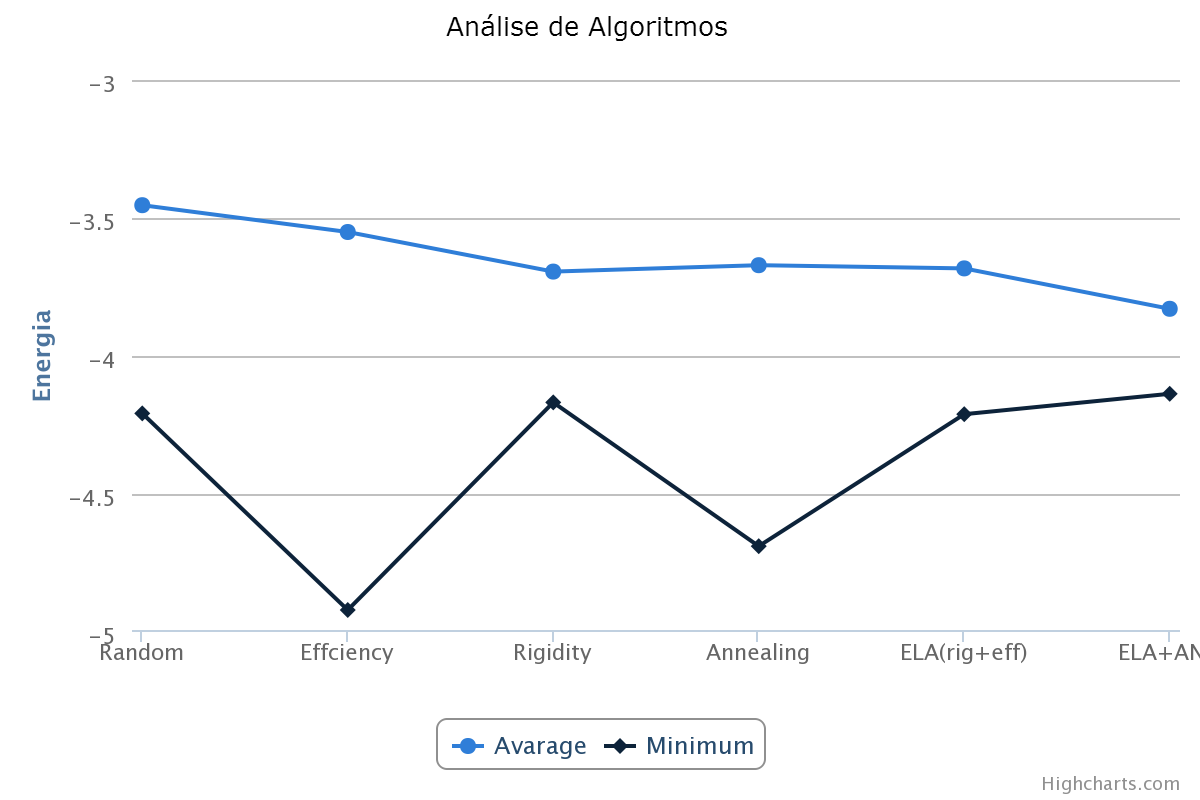
\includegraphics[scale=.3]{img/analise.png}
\caption{Análise dos resultados de testes para a sequência FIBO7(21).} 
\label{analise}
\end{figure}
  
Observa-se, pela média, que todos os conceitos contribuem para melhorar os resultados obtidos, porém nem sempre o mínimo encontrado em cada conjunto de testes acompanha a média dos resultados dos testes. O refinamento através do algoritmo ANN contribui tanto para os resultados quanto a utilização em conjunto dos dois conceitos (Rigidez e Eficiência) do algoritmo ELA. O melhor resultado foi obtido através da execução de ambos algoritmos atuando em série (Figura \ref{analise}).

A calibragem dos parâmetros que alteram os valores de Rigidez e Eficiência em caso de sucesso (modelo mais estável) ou falha é fundamental para que o algoritmo ELA obtenha bons reultados. Esses parâmetros são analisados de forma independente para a eficiência e foram gerados os gráficos que demonstram sua relação. Nas figuras \ref{effheatmin} e \ref{effheatavg} é possível vizualizar as relações entre os parâmetros e os resultados obtidos.

\begin{figure}[htbp]
  \centering 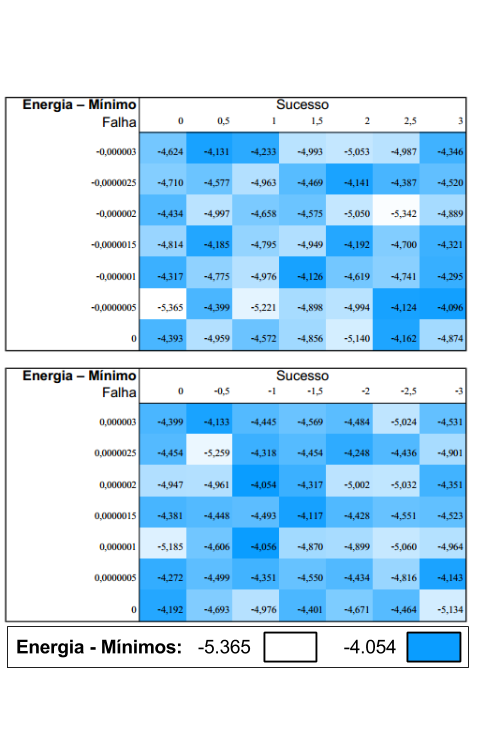
\includegraphics[scale=.6]{img/effheatmin.png}
\caption{Energia mínima em relação aos parâmetros que alteram a eficiência.} 
\label{effheatmin}
\end{figure}

\begin{figure}[htbp]
  \centering 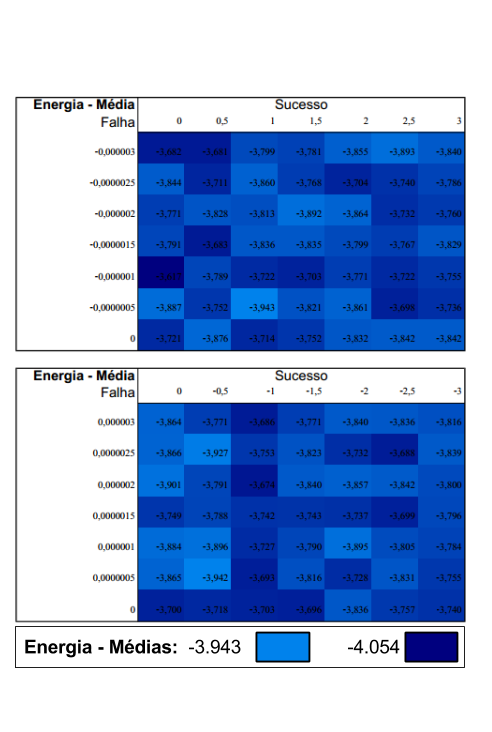
\includegraphics[scale=.6]{img/effheatavg.png}
\caption{Energia média em relação aos parâmetros alteram a eficiência.} 
\label{effheatavg}
\end{figure}

Um valor positivo para o parâmetro relacionado à Eficiência em caso de sucesso, significa que, caso uma dobra naquele ângulo resulte em um modelo mais estável, a chance de selecionar novamente o mesmo ângulo será maior. No caso desse mesmo valor ser negativo, a chance de voltarmos à este aminoácido será menor.

De forma análoga, se o parâmetro relacionado à Rigidez em caso de sucesso for definido como positivo, em uma dobra bem sucedida, a Rigidez deste ângulo aumentará. Valores negativos para este parâmetro tornarão os ângulos mais flexíveis quando forem encontrados modelos mais estáveis.

Os valores para casos de falha são consideravelmente menores que os de sucesso devido ao fato de obtermos um número pequeno de sucessos em um novo conjunto de soluções. Desta forma, os valores são alterados diversas vezes com incrementos pequenos (falhas) e, nas soluções de sucesso, os valores maiores fazem a compensação. Se não houver esse equilíbrio, os valores dos parâmetros não serão alterados na maior parte dos resultados pois terão atingido seu limite. Os valores precisam estar equilibrados para cumprirem sua função na busca. 

Observa-se através do gráfico das médias da Figura \ref{effheatavg} que o valor ideal para essa sequência é de 1 para os casos de sucesso e de 0,0000005 para os casos de falha. Porém esses valores também têm relação com outros parâmetros e seu desempenho pode mudar para outras sequências.

Quando é realizada uma alteração no valor da Rigidez de um ângulo, também são alterados um número determinado de vizinhos. Determinar esse número de vizinhos e como são alterados seus valores é possível através de parâmetros específicos. A análise desse número de vizinhos, de 0 à 6 vizinhos afetados pela Rigidez, é apresentada na Figura \ref{rigv}. Foi utilizada uma expressão linear para distribuir essa alteração porém outras formas de distribuição poderiam ser utilizadas. 

Para a sequência testada, de acordo com a média, o valor ideal de vizinhos é de três. Esse número de vizinhos a alterar é um valor que está provavelmente relacionado diretamente ao comprimento da cadeia primária. Outras propriedades da cadeia também podem influenciar no valor ideal para este parâmetro como o número de aminoácidos consecutivos de mesmo tipo. 

\begin{figure}[htbp]
  \centering 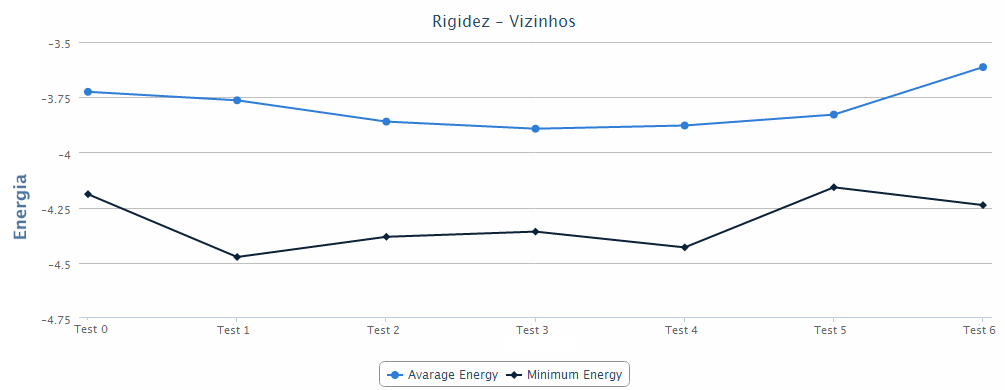
\includegraphics[scale=.43]{img/rigv.png}
\caption{Análise do número de vizinhos afetados pela Rigidez.} 
\label{rigv}
\end{figure}

A seguir são apresentadas na Figura \ref{finalchart} as comparações dos resultados encontrados neste trabalho com os de outros trabalhos contemporâreos que compartilham do mesmo modelo. Para os algoritmos ACMC, STMD e CSA não foram encontrados resultados com as cadeias baseadas em proteinas reais. 

À partir da análise dos resultados descritos na Tabela \ref{results}, pode-se notar que para as proteínas com as sequências FIBO6(13), FIBO7(21) e FIBO8(34) os resultados do algoritmo proposto (ELA+ANN) se assemelha aos da literatura.

A única cadeia que não apresentou um resultado satisfatório foi Fibonacci 9, talvez um dos motivos desse resultado inferior seja o fato dessa ser uma cadeia longa, com 55 aminoácidos. Para a proteína real adaptada 1AHO, de 64 aminoácidos apresentou um resultado satisfatório. O tempo necessário para testes nessas cadeias mais longas é consideravelmente maior, o que torna mais difícil sua calibragem de parâmetros e diminui a quantidade de testes realizados.

O resultado obtido na proteína 1AGT foi o menor, mesmo quando comparado com os de algoritmos que são evoluções de métodos conhecidos. Esse resultado demonstra que os métodos propostos são promissores e que seu estudo pode gerar resultados ainda melhores.

\begin{figure}[htbp]
  \centering 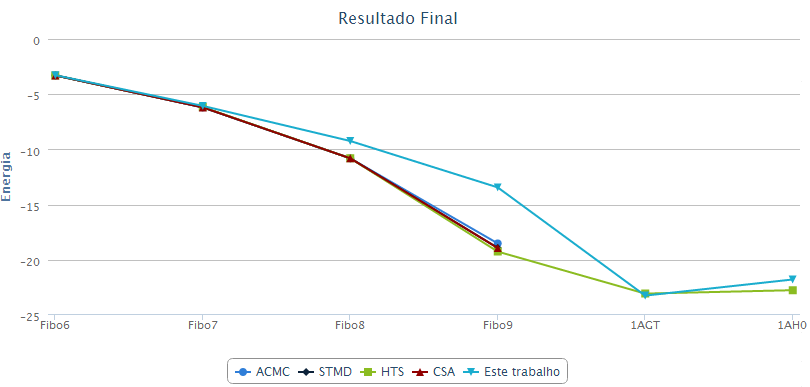
\includegraphics[scale=.65]{img/finalchart.png}
\caption{Comparação de resultados em gráfico} 
\label{finalchart}
\end{figure}

\begin{table}
\begin{center}
\caption{Comparação de resultados atuais}\label{results}
\begin{tabular}{lccccr}
\hline
Cadeia & ACMC \cite{liang2004annealing} & STMD \cite{kim2006statistical} & HTS \cite{liu2013heuristic} & CSA \cite{lee2008re} & ELA+ANN (Proposta) \\
\hline
FIBO6(13) & -3.2941 & -3.2941 & -3.2941 & -3.2941 & -3.27562491074513\\
FIBO7(21) & -6.1976 & -6.1980 & -6.1680 & -6.1980 & -6.0578768984653\\
FIBO8(34) & -10.8060 & -10.8060 & -10.8060 & -10.8060 & -9.23852675468751\\
FIBO9(55) & -18.7407 & -18.9202 & -19.257 & -18.9296 & -13.441023912647\\
1AGT(34) & - & - & -23.0575 & - & -23.2433303926769\\
1AHO(64) & - & - & -22.7554 & - & -21.7818222352442\\
\hline
\end{tabular}
\end{center}
\end{table}

Finalmente apresentamos as melhores soluções obtidas com a aplicação na Figura \ref{finalrender}. É possível visualizar, em especial no modelo 1AGT, padrões de dobra similares aos de proteínas reais e a formação de núcleos hidrofóbicos (A).

\begin{figure}[htbp]
  \centering 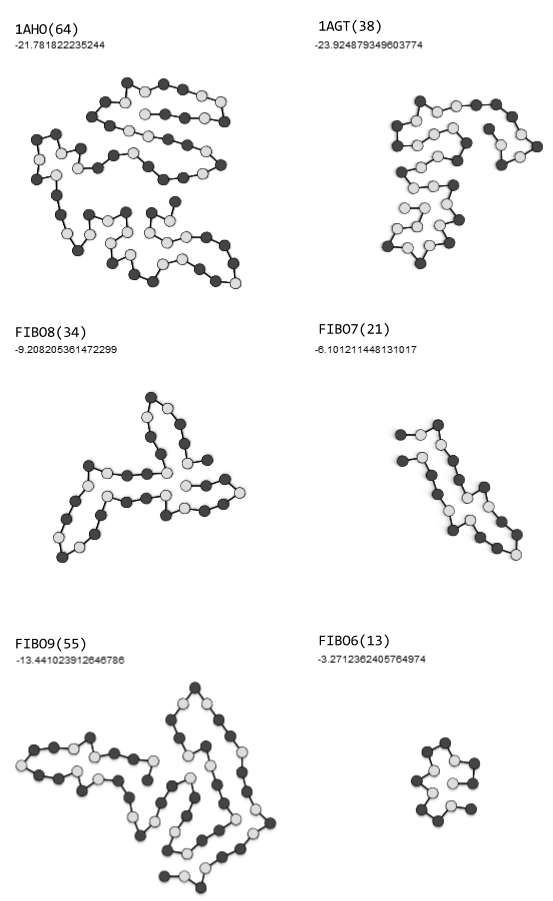
\includegraphics[scale=.7]{img/finalrender.png}
\caption{Renderização dos modelos mais estáveis encontrados.} 
\label{finalrender}
\end{figure}

\chapter{Conclusão}

Nesse trabalho é proposto um algoritmo para dobramento de proteínas no Modelo AB. O trabalho aponta diversas áreas para pesquisas futuras que podem tornar a proposta mais abrangente. 

É necessário analisar questões relacionadas à implementação, pois é provável que existam outras abordagens que otimizem a performance dos algoritmos. Também é preciso avaliar corretamente os interpretadores em $Javascript$ e realizar experimentos com {\it benchmarks} para adquirir maior conhecimento e confiabilidade neste tipo de implementação. Todos os testes apresentados foram realizados com a {\it Engine V8 - WebKit} no {\it navegador Chrome} e os arquivos servidos pelo {\it Nodejs}. É importante ressaltar que diferentes interpretadores podem alterar a performance e a execução da aplicação.

Em relação aos algoritmos, percebe-se ainda a necessidade de uma análise mais detalhada das combinações de todos os parâmetros, para determinar os valores ideais de execução. É preciso relacionar essa análise em diferentes comprimentos de proteína para determinar quais tem relação direta com esse comprimento e que tipo de relação existe.

Apesar dos resultados serem muito importantes para a proposta, o que se espera é validar as técnicas propostas e no futuro combiná-las com outras, gerando heurísticas de alto nível que possam ser utilizadas em outros problemas complexos. 

Todo o código fonte da aplicação e seus algoritmos apresentados neste trabalho estão dísponíveis através do repositório ({\it https://github.com/rafaelcastrocouto/initio}). A API está documentada e armazenada no subdiretório “$docs$” e pode ser utilizada para expandir as capacidades da aplicação para execução de experimentos e dos algoritmos.

Como trabalhos futuros, propõe-se, além das análises mencionadas, a exploração de outras técnicas em conjunto com as propostas, com o objetivo de melhorar ainda mais os resultados. Devido ao fato de ser desenvolvida em $Javascript$, a aplicação torna muito simples o desenvolvimento de estratégias para a execução paralela, tanto com processos na mesma máquina ({\it workers}) quanto com a distribuição da execução da aplicação na rede. Tirar proveito destas possibilidades implicaria em uma grande contribuição para a proposta.

Ressalte-se que a proposta aqui apresentada se restringe à geração consecutiva de novas soluções baseada somente nos parâmetros, sem armazenar dados de conjuntos de testes anteriores em memória. Portanto, outra grande contribuição será a implementação de algoritmos que façam uso desses dados e que estabelaçam entre eles possíveis relações. Essas abordagens podem ser aplicadas tando para os resultados (sequência de ângulos) quanto para os valores de Rigidez e Eficiência.

Outra contribuição significativa para a proposta seria a integração com os algoritmos que utilizam outras técnicas como clusterizações, cruzamentos, além de outros métodos de refinamento mais eficiêntes.

\bibliographystyle{plain}
\nocite{*}
\bibliography{references}
\end{document}